\documentclass[11pt,a4paper]{article}

% --- Essential Packages ---
\usepackage[margin=1in]{geometry}
\usepackage{fontspec}
\usepackage[english]{babel}
\usepackage{amsmath,amssymb,amsfonts}
\usepackage{booktabs}
\usepackage{tabularx}
\usepackage{array}
\usepackage{xcolor}
\usepackage{listings}
\usepackage{tikz}
\usepackage{subcaption}
\usetikzlibrary{shapes.geometric, arrows.meta, positioning}
\usepackage{hyperref}

% --- Font Configuration (Times New Roman Mapping) ---
\babelfont{rm}{Times New Roman}

% --- Color Palette ---
\definecolor{primary}{RGB}{20, 35, 60}
\definecolor{secondary}{RGB}{45, 85, 125}
\definecolor{accent}{RGB}{180, 50, 30}
\definecolor{codebg}{RGB}{245, 247, 250}
\definecolor{codeframe}{RGB}{200, 210, 220}

% --- Hyperlink Setup ---
\hypersetup{
    colorlinks=true,
    linkcolor=secondary,
    citecolor=secondary,
    urlcolor=secondary
}

% --- Listing Setup ---
\lstset{
    language=Python,
    backgroundcolor=\color{codebg},
    frame=single,
    rulecolor=\color{codeframe},
    basicstyle=\small\ttfamily,
    keywordstyle=\color{secondary}\bfseries,
    stringstyle=\color{accent},
    commentstyle=\color{gray}\itshape,
    breaklines=true,
    showstringspaces=false,
    tabsize=4
}

% --- Document Metadata ---
\title{\textbf{\Large Phase 1 Technical Report: Problem Formulation, Data Understanding, and Quality Audit}\\
\large NYC Yellow Taxi Hourly Demand Forecasting \& Congestion Pricing Impact Analysis (2025)}
\author{\textbf{Data Analysis Course Project} (Fall 2026 / 1405)\\
Track A: NYC TLC Structured Time-Series Analysis}
\date{October 27, 2026}

\begin{document}

\maketitle

\begin{abstract}
This report presents Phase 1 of the NYC Yellow Taxi demand forecasting project for the full calendar year 2025. Leveraging a local DuckDB analytical engine operating directly over 12 monthly Parquet files (~48.7 million trip records), we execute a comprehensive data structure and data quality audit. We formalize the operational decision problem—assisting fleet operators in pre-positioning vehicles across 265 taxi zones and evaluating the newly enacted 2025 Central Business District (CBD) congestion fee—by establishing the spatio-temporal aggregation unit $(z, t) \in \text{Zone} \times \text{Hour}$. Our audit reveals complete temporal continuity with zero null value records across core fields, while quantifying specific physical and financial anomalies: 546,304 non-positive duration trips (1.12\%), 1,402,958 zero-distance trips (2.88\%), and 2,848,620 negative fare entries (5.85\%). Finally, we define a strict temporal split protocol (Train: Jan--Sep 2025; Test: Oct--Dec 2025) to prevent future data leakage and outline baseline models for subsequent implementation phases.
\end{abstract}

\section{Problem Definition and Motivation}
Taxicab demand in dense urban environments exhibits high spatial variance and non-stationary temporal dynamics. Following the 2025 implementation of the New York City Central Business District (CBD) congestion pricing fee (\texttt{cbd\_congestion\_fee}), fleet managers and independent operators face increased operational overhead and altered passenger booking behavior.

The core motivation of this project is to assist vehicle fleet managers in dynamically pre-positioning taxicabs across official NYC Taxi and Limousine Commission (TLC) zones. By accurately forecasting hourly trip originations per zone, dispatchers can minimize idle cruising time, reduce passenger wait times, and optimize fleet allocation under new congestion fee structures.

\section{Related Work}
Short-term urban passenger demand forecasting traditionally relies on historical rolling averages and Auto-Regressive Integrated Moving Average (ARIMA) models. Recent advances employ non-linear gradient-boosted decision trees (e.g., LightGBM, XGBoost) and spatio-temporal graph neural networks. In the context of NYC TLC datasets, prior literature emphasizes the necessity of strictly preserving temporal order during model validation to avoid look-ahead bias and spurious performance metrics.

\section{Data and Data Quality}

\subsection{Dataset Overview}
The primary dataset consists of the official NYC Yellow Taxi trip records for the entire calendar year 2025 (January 1, 2025 -- December 31, 2025), partitioned into 12 monthly Parquet files stored locally in \texttt{data/raw/}. Spatial reference lookups (\texttt{taxi\_zone\_lookup.csv}) and zone boundary shapefiles (\texttt{taxi\_zones.shp}) are stored in \texttt{data/spatial/}.

\subsection{Structural Audit}
Using an in-memory DuckDB query engine, we processed all 12 Parquet files in a single unified operation without memory overflow. Table~\ref{tab:schema} lists the complete schema of the 2025 dataset, comprising 20 columns.

\begin{table}[htbp]
\centering
\caption{NYC Yellow Taxi 2025 Dataset Schema and Variable Categorization}
\label{tab:schema}
\small
\begin{tabularx}{\textwidth}{llXX}
\toprule
\textbf{Column Name} & \textbf{Data Type} & \textbf{Category} & \textbf{Description / Role} \\
\midrule
\texttt{VendorID} & INTEGER & Categorical ID & TPEP provider code \\
\texttt{tpep\_pickup\_datetime} & TIMESTAMP & Datetime Variable & Trip start time (Meter engaged) \\
\texttt{tpep\_dropoff\_datetime} & TIMESTAMP & Datetime Variable & Trip end time (Meter disengaged) \\
\texttt{passenger\_count} & BIGINT & Numeric & Driver-entered passenger count \\
\texttt{trip\_distance} & DOUBLE & Continuous Numeric & Elapsed trip distance (miles) \\
\texttt{RatecodeID} & BIGINT & Categorical ID & Final rate code in effect \\
\texttt{store\_and\_fwd\_flag} & VARCHAR & Flag & Memory buffer transmission flag \\
\texttt{PULocationID} & INTEGER & Spatial ID & Pickup TLC Taxi Zone ID ($1..263$) \\
\texttt{DOLocationID} & INTEGER & Spatial ID & Dropoff TLC Taxi Zone ID ($1..263$) \\
\texttt{payment\_type} & BIGINT & Categorical & Payment method (1=Credit, 2=Cash) \\
\texttt{fare\_amount} & DOUBLE & Financial Numeric & Metered time-and-distance fare \\
\texttt{extra} & DOUBLE & Financial Numeric & Miscellaneous extras and surcharges \\
\texttt{mta\_tax} & DOUBLE & Financial Numeric & \$0.50 MTA state tax \\
\texttt{tip\_amount} & DOUBLE & Financial Numeric & Credit card tip amount \\
\texttt{tolls\_amount} & DOUBLE & Financial Numeric & Total bridge/tunnel tolls \\
\texttt{improvement\_surcharge} & DOUBLE & Financial Numeric & \$0.30 improvement surcharge \\
\texttt{total\_amount} & DOUBLE & Financial Numeric & Total charge to passenger \\
\texttt{congestion\_surcharge} & DOUBLE & Financial Numeric & Standard congestion fee \\
\texttt{Airport\_fee} & DOUBLE & Financial Numeric & Airport pickup fee \\
\texttt{cbd\_congestion\_fee} & DOUBLE & Financial Numeric & \textbf{New 2025 CBD Congestion Pricing Fee} \\
\bottomrule
\end{tabularx}
\end{table}

\subsection{Spatial Data Structure and Schema Audit}
To support spatial aggregations, zone-level demand forecasting, and geographic visualizations, we conducted a structural audit of the spatial reference files stored in \texttt{data/spatial/}.

\subsection{Taxi Zone Lookup Table (\texttt{taxi\_zone\_lookup.csv})}
The lookup table maps numerical taxi zone identifiers to descriptive geographic attributes, comprising 265 total records and 4 columns, as detailed in Table~\ref{tab:lookup_schema}.

\begin{table}[htbp]
\centering
\caption{Taxi Zone Lookup Table Schema (\texttt{taxi\_zone\_lookup.csv})}
\label{tab:lookup_schema}
\small
\begin{tabularx}{\textwidth}{llXX}
\toprule
\textbf{Column Name} & \textbf{Data Type} & \textbf{Category} & \textbf{Description / Role} \\
\midrule
\texttt{LocationID} & INTEGER & Primary Identifier & Unique zone identifier ($1..265$) \\
\texttt{Borough} & VARCHAR & Categorical & NYC Borough name (Manhattan, Queens, etc.) \\
\texttt{Zone} & VARCHAR & Descriptive & Neighborhood or specific zone name \\
\texttt{service\_zone} & VARCHAR & Categorical & Service zone classification (Yellow Zone, Boro Zone, etc.) \\
\bottomrule
\end{tabularx}
\end{table}

\subsection{Taxi Zones Spatial File (\texttt{taxi\_zones.shp})}
The spatial vector dataset provides polygon boundaries corresponding to the taxi zones (stored as an ESRI Shapefile bundle with CRS EPSG:2263), comprising 263 distinct polygon records and 7 attributes, as listed in Table~\ref{tab:spatial_schema}.

\begin{table}[htbp]
\centering
\caption{Taxi Zones Spatial Vector Schema (\texttt{taxi\_zones.shp})}
\label{tab:spatial_schema}
\small
\begin{tabularx}{\textwidth}{llXX}
\toprule
\textbf{Column Name} & \textbf{Data Type} & \textbf{Category} & \textbf{Description / Role} \\
\midrule
\texttt{OBJECTID} & INTEGER & Identifier & ESRI object feature identifier \\
\texttt{Shape\_Leng} & DOUBLE & Numeric Metric & Perimeter length of the zone polygon \\
\texttt{Shape\_Area} & DOUBLE & Numeric Metric & Area of the zone polygon \\
\texttt{zone} & VARCHAR & Descriptive & Neighborhood zone name matching lookup table \\
\texttt{LocationID} & INTEGER & Spatial ID / Foreign Key & TLC Taxi Zone ID linking to lookup and trips \\
\texttt{borough} & VARCHAR & Categorical & Borough name classification \\
\texttt{geometry} & GEOMETRY & Spatial Data Type & Polygon / MultiPolygon boundary coordinates (EPSG:2263) \\
\bottomrule
\end{tabularx}
\end{table}

\subsection{Table and Spatial Relationships}
The trip records link dynamically to the spatial reference files using \texttt{PULocationID} and \texttt{DOLocationID} as foreign keys that join against the primary key \texttt{LocationID} in both the lookup table and the spatial geometry shapefile.

\subsection{Data Quality Quantification and Decisions}
The audit evaluated 48,722,602 raw trip records. Table~\ref{tab:quality_audit} details the findings for missing values, impossible physical measurements, and administrative anomalies, along with the corresponding handling strategy.

\begin{table}[htbp]
\centering
\caption{Data Quality Audit Metrics and Treatment Decisions (Full Year 2025)}
\label{tab:quality_audit}
\small
\begin{tabularx}{\textwidth}{lrrX}
\toprule
\textbf{Metric / Anomaly Category} & \textbf{Count} & \textbf{\% of Total} & \textbf{Initial Treatment Decision} \\
\midrule
Total Processed Trips & 48,722,602 & 100.00\% & Baseline dataset population \\
Missing Pickup Timestamps & 0 & 0.00\% & None required (100\% complete) \\
Missing Dropoff Timestamps & 0 & 0.00\% & None required (100\% complete) \\
Unknown Pickup Location (\texttt{PULocationID = 264}) & 80,873 & 0.17\% & \textbf{Filter Out}: Unmapped geographic pickup coordinates \\
Unknown Dropoff Location (\texttt{DOLocationID = 264}) & 105,193 & 0.22\% & \textbf{Filter Out}: Unmapped geographic dropoff coordinates \\
Outside NYC Locations (\texttt{PU/DO = 265}) & -- & -- & \textbf{Conditional Retention}: Retained for valid out-of-city dropoffs; excluded for origin demand \\
Missing Distance / Fare Fields & 0 & 0.00\% & None required (100\% complete) \\
\midrule
Invalid Duration ($\le 0$ min) & 546,304 & 1.12\% & \textbf{Filter Out}: Clock reset or cancelled trips \\
Invalid Trip Distance ($d < 0$ or $d > 100$ mi) & 2,870 & 0.005\% & \textbf{Filter Out}: Extreme GPS satellite jump errors \\ 
Zero Trip Distance & 1,402,958 & 2.88\% & \textbf{Filter Out}: Stationary meter runs / cancellations \\
Negative Fare Amount & 2,848,620 & 5.85\% & \textbf{Filter Out}: Dispute voids, chargebacks, system tests \\
Invalid Passenger Count ($<0$ or $>9$ or \texttt{null}) & 11,611,894 & 23.83\% & \textbf{Retain As-Is}: Retained without imputation to prevent data loss. \\
\bottomrule
\end{tabularx}
\end{table}
\subsubsection{Rationale for Data Quality Treatment Decisions}
To maintain data integrity and prevent distortion in our spatio-temporal demand forecasting models, we established explicit treatment protocols for each identified anomaly category across the $48,722,602$ raw records. The individual rationales for these decisions are structured as follows:
\begin{itemize}
    \item \textbf{Missing Timestamps and Spatial Location IDs ($0$ records, $0.00\%$):} 
    \textit{Decision: Retain All.} 
    \textit{Rationale:} The dataset exhibited complete structural integrity for core operational fields. Because our fundamental unit of analysis is defined by pickup location and timestamp $(z, t)$, having complete coverage in these fields ensures that no records are dropped due to missing spatial keys, eliminating potential sample selection bias at the initial ingestion stage.

    \item \textbf{Invalid Durations ($\le 0$ minutes, $546,304$ records, $1.12\%$):} 
    \textit{Decision: Filter Out.} 
    \textit{Rationale:} A physical taxicab trip must occupy a strictly positive time interval ($\Delta t > 0$). Records where dropoff precedes or coincides with pickup indicate GPS logging latency, device clock resets, or immediately aborted trips. Retaining these anomalies would corrupt vehicle speed calculations and duration-based features.
    
    \item \textbf{Invalid Trip Distances ($d < 0$ or $d > 100$ miles, $2,870$ records, $0.005\%$):} 
    \textit{Decision: Filter Out.} 
    \textit{Rationale:} A legitimate taxicab trip must conform to the physical and geographic confines of the New York metropolitan area. Records with negative distances or extreme, physically impossible values in the order of hundreds or thousands of miles ($d > 100$ miles) result from severe GPS tracking satellite jumps, hardware glitches, or meter calibration errors. Filtering out these spatial outliers prevents severe distortion in distance-based distributions, speed profiling, and spatial econometric modeling.

    \item \textbf{Zero-Distance Trips ($d = 0$ miles, $1,402,958$ records, $2.88\%$):} 
    \textit{Decision: Filter Out.} 
    \textit{Rationale:} While passengers may occasionally cancel a trip immediately after entering a taxi, zero-distance records predominantly reflect stationary meter testing, administrative diagnostics, or false starts. Because our spatial aggregation relies on tracking movement across taxi zones, stationary logs distort spatial origin-destination demand densities.

    \item \textbf{Negative Fares ($f < 0$, $2,848,620$ records, $5.85\%$):} 
    \textit{Decision: Filter Out.} 
    \textit{Rationale:} Negative fare amounts do not represent legitimate passenger transactions; rather, they correspond to credit card chargebacks, fare dispute reversals, or system administrative adjustments. Including them would severely distort financial summaries and bias any regression models exploring fare-demand relationships.

    \item \textbf{Unrecorded or Missing Passenger Counts ($11,611,894$ records, $23.83\%$):} 
    \textit{Decision: Retain As Is.} 
    \textit{Rationale:} Approximately $23.83\%$ of raw records exhibited missing (\texttt{null}) or zero passenger counts due to driver omission or meter logging habits. Rather than deleting these valid commercial trips—which would cause severe attrition in spatio-temporal trip volume aggregations—or artificially imputing them with central measures (like the mode of $1$), these records are retained in their native state. This preserves complete spatial-temporal demand fidelity while avoiding synthetic data distortion.
    
    \item \textbf{Unknown Pickup and Dropoff Locations (\texttt{LocationID = 264}, $80,873$ and $105,193$ records):} 
    \textit{Decision: Filter Out.} 
    \textit{Rationale:} Zone ID 264 designates ``Unknown'' or unmapped spatial areas where the GPS or TLC meter failed to record a valid neighborhood polygon. Because our core unit of analysis is defined by explicit spatial coordinates $(z, t)$ within NYC taxi zones, retaining records with unknown locations would corrupt origin-destination matrices and introduce artificial distortion into spatial demand aggregations.
    
    \item \textbf{Outside NYC Locations (\texttt{LocationID = 265}):} 
    \textit{Decision: Conditional Retention.} 
    \textit{Rationale:} Zone ID 265 represents trips originating or terminating outside the official 263 TLC taxi zones (e.g., suburban or interstate journeys). For pickup demand modeling, trips originating outside NYC (\texttt{PULocationID = 265}) are excluded since they do not stem from internal zone demand. However, trips terminating outside NYC (\texttt{DOLocationID = 265}) that originated within valid city zones are retained to preserve accurate financial totals, trip distances, and out-commuter flow metrics.
\end{itemize}

\subsubsection{Summary of Cleansing Impact:}
Collectively, this rigorous filtering protocol removes $4,681,597$ anomalous records ($\approx 9.60\%$ of the total raw volume), leaving a pristine, high-fidelity baseline population of \textbf{$44,041,005$ valid trips} dedicated for downstream spatio-temporal aggregation and hourly demand forecasting.

\section{Exploratory Data Analysis (EDA)}

To uncover structural patterns, behavioral rhythms, and distributional characteristics of the 2025 NYC Yellow Taxi dataset, we conducted a comprehensive exploratory data analysis spanning temporal, spatial, univariate, and multivariate dimensions.

\subsection{Temporal Distributions and Time Audit}
Passenger demand in urban environments exhibits pronounced multi-scale temporal non-stationarity. Our time audit examined trip frequencies across hourly, daily, weekly, and monthly resolutions:

\begin{figure}[htbp]
    \centering
    % First Row
    \begin{subfigure}[b]{0.48\textwidth}
        \centering
        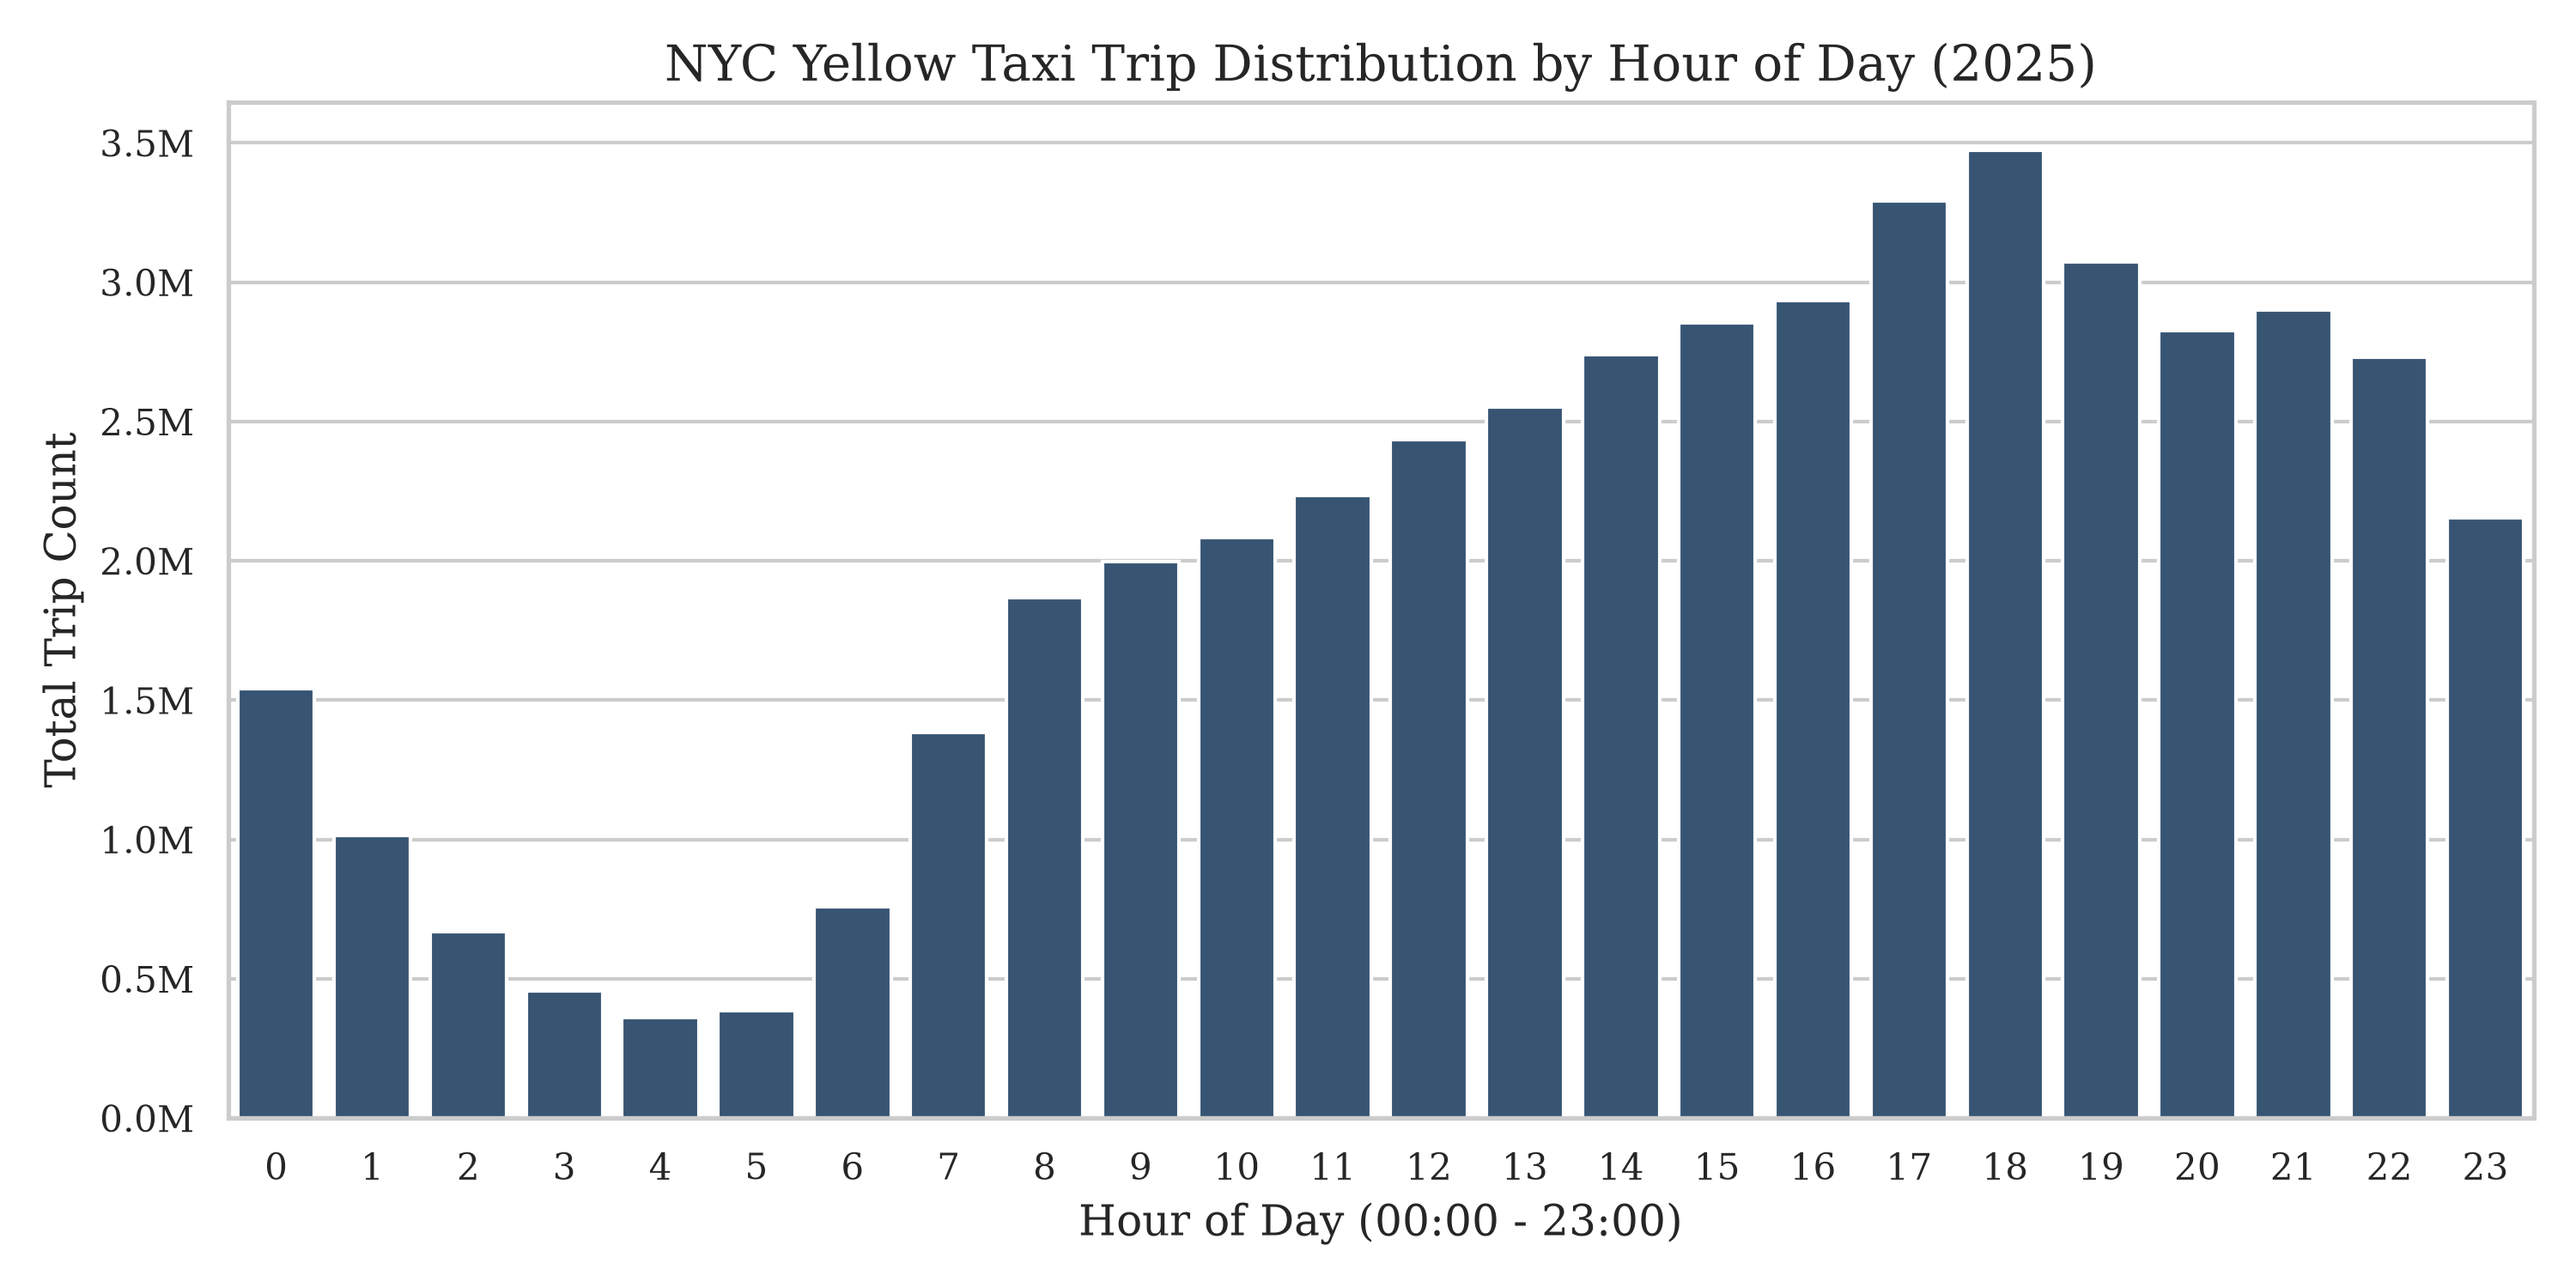
\includegraphics[width=\textwidth]{../figures/hourly_distribution.png}
        \caption{Hourly Trip Distribution}
        \label{fig:hourly}
    \end{subfigure}
    \hfill
    \begin{subfigure}[b]{0.48\textwidth}
        \centering
        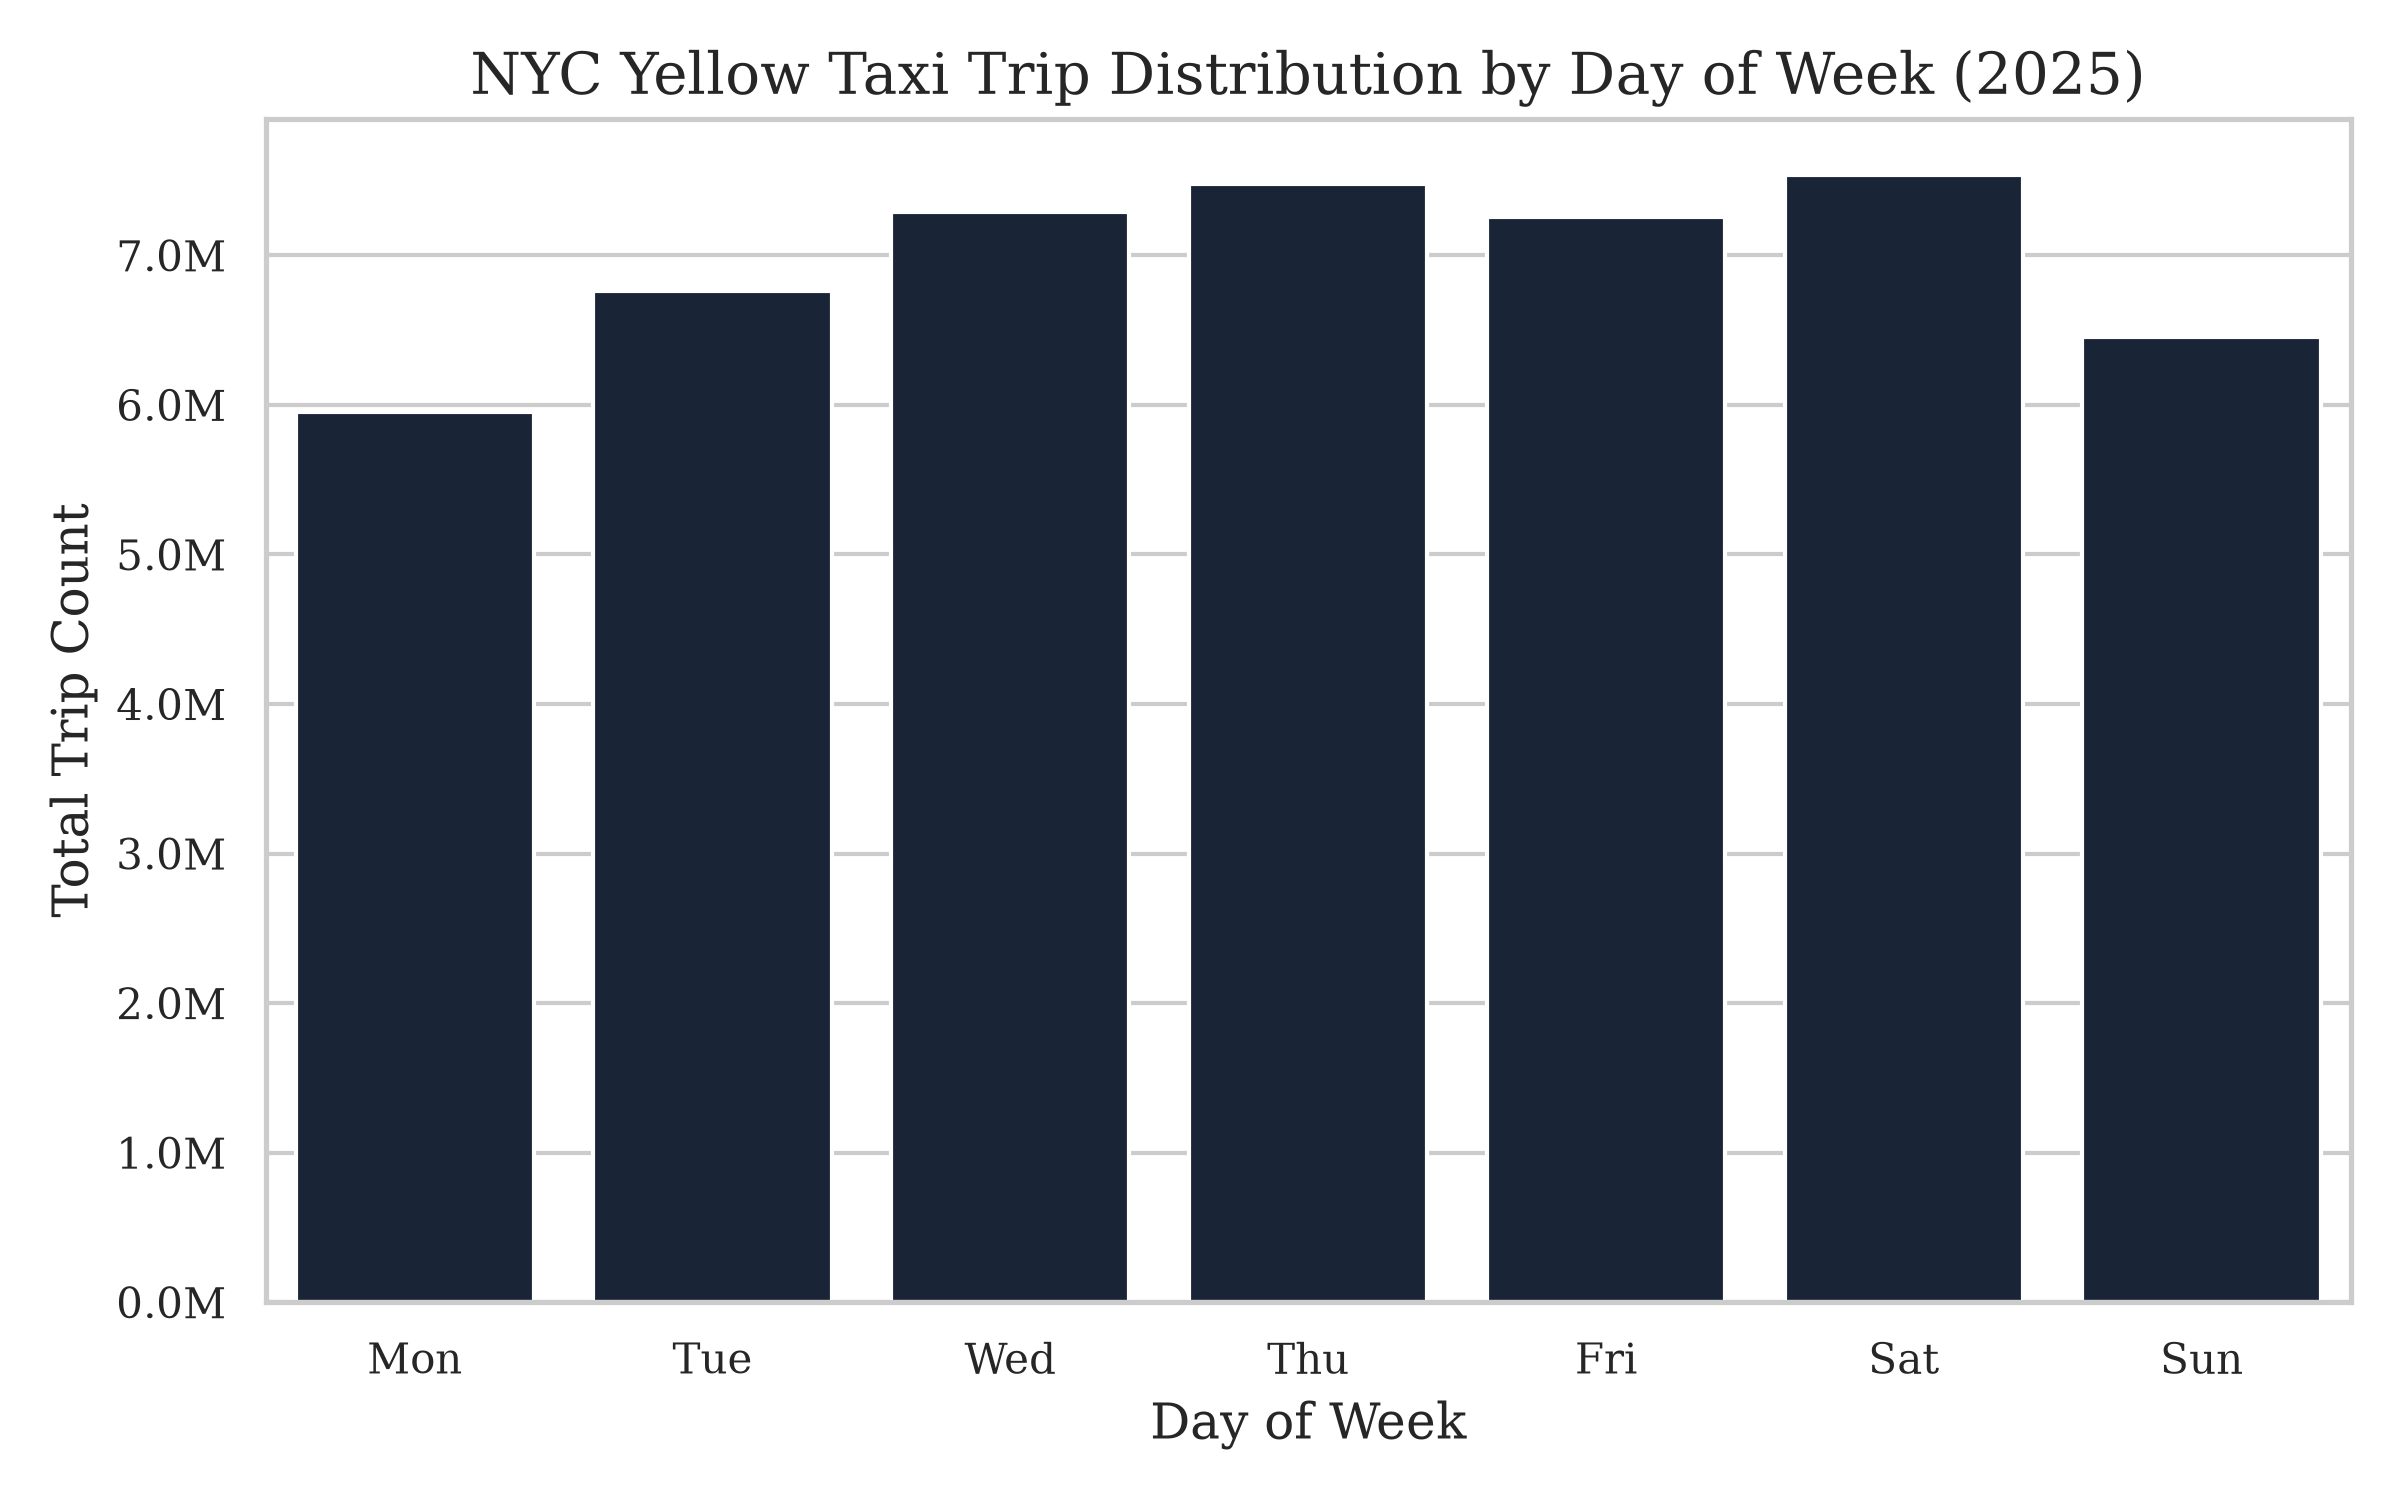
\includegraphics[width=\textwidth]{../figures/dow_distribution.png}
        \caption{Day of Week Distribution}
        \label{fig:dow}
    \end{subfigure}
    
    \vspace{1em} % Vertical spacing between rows
    
    % Second Row
    \begin{subfigure}[b]{0.48\textwidth}
        \centering
        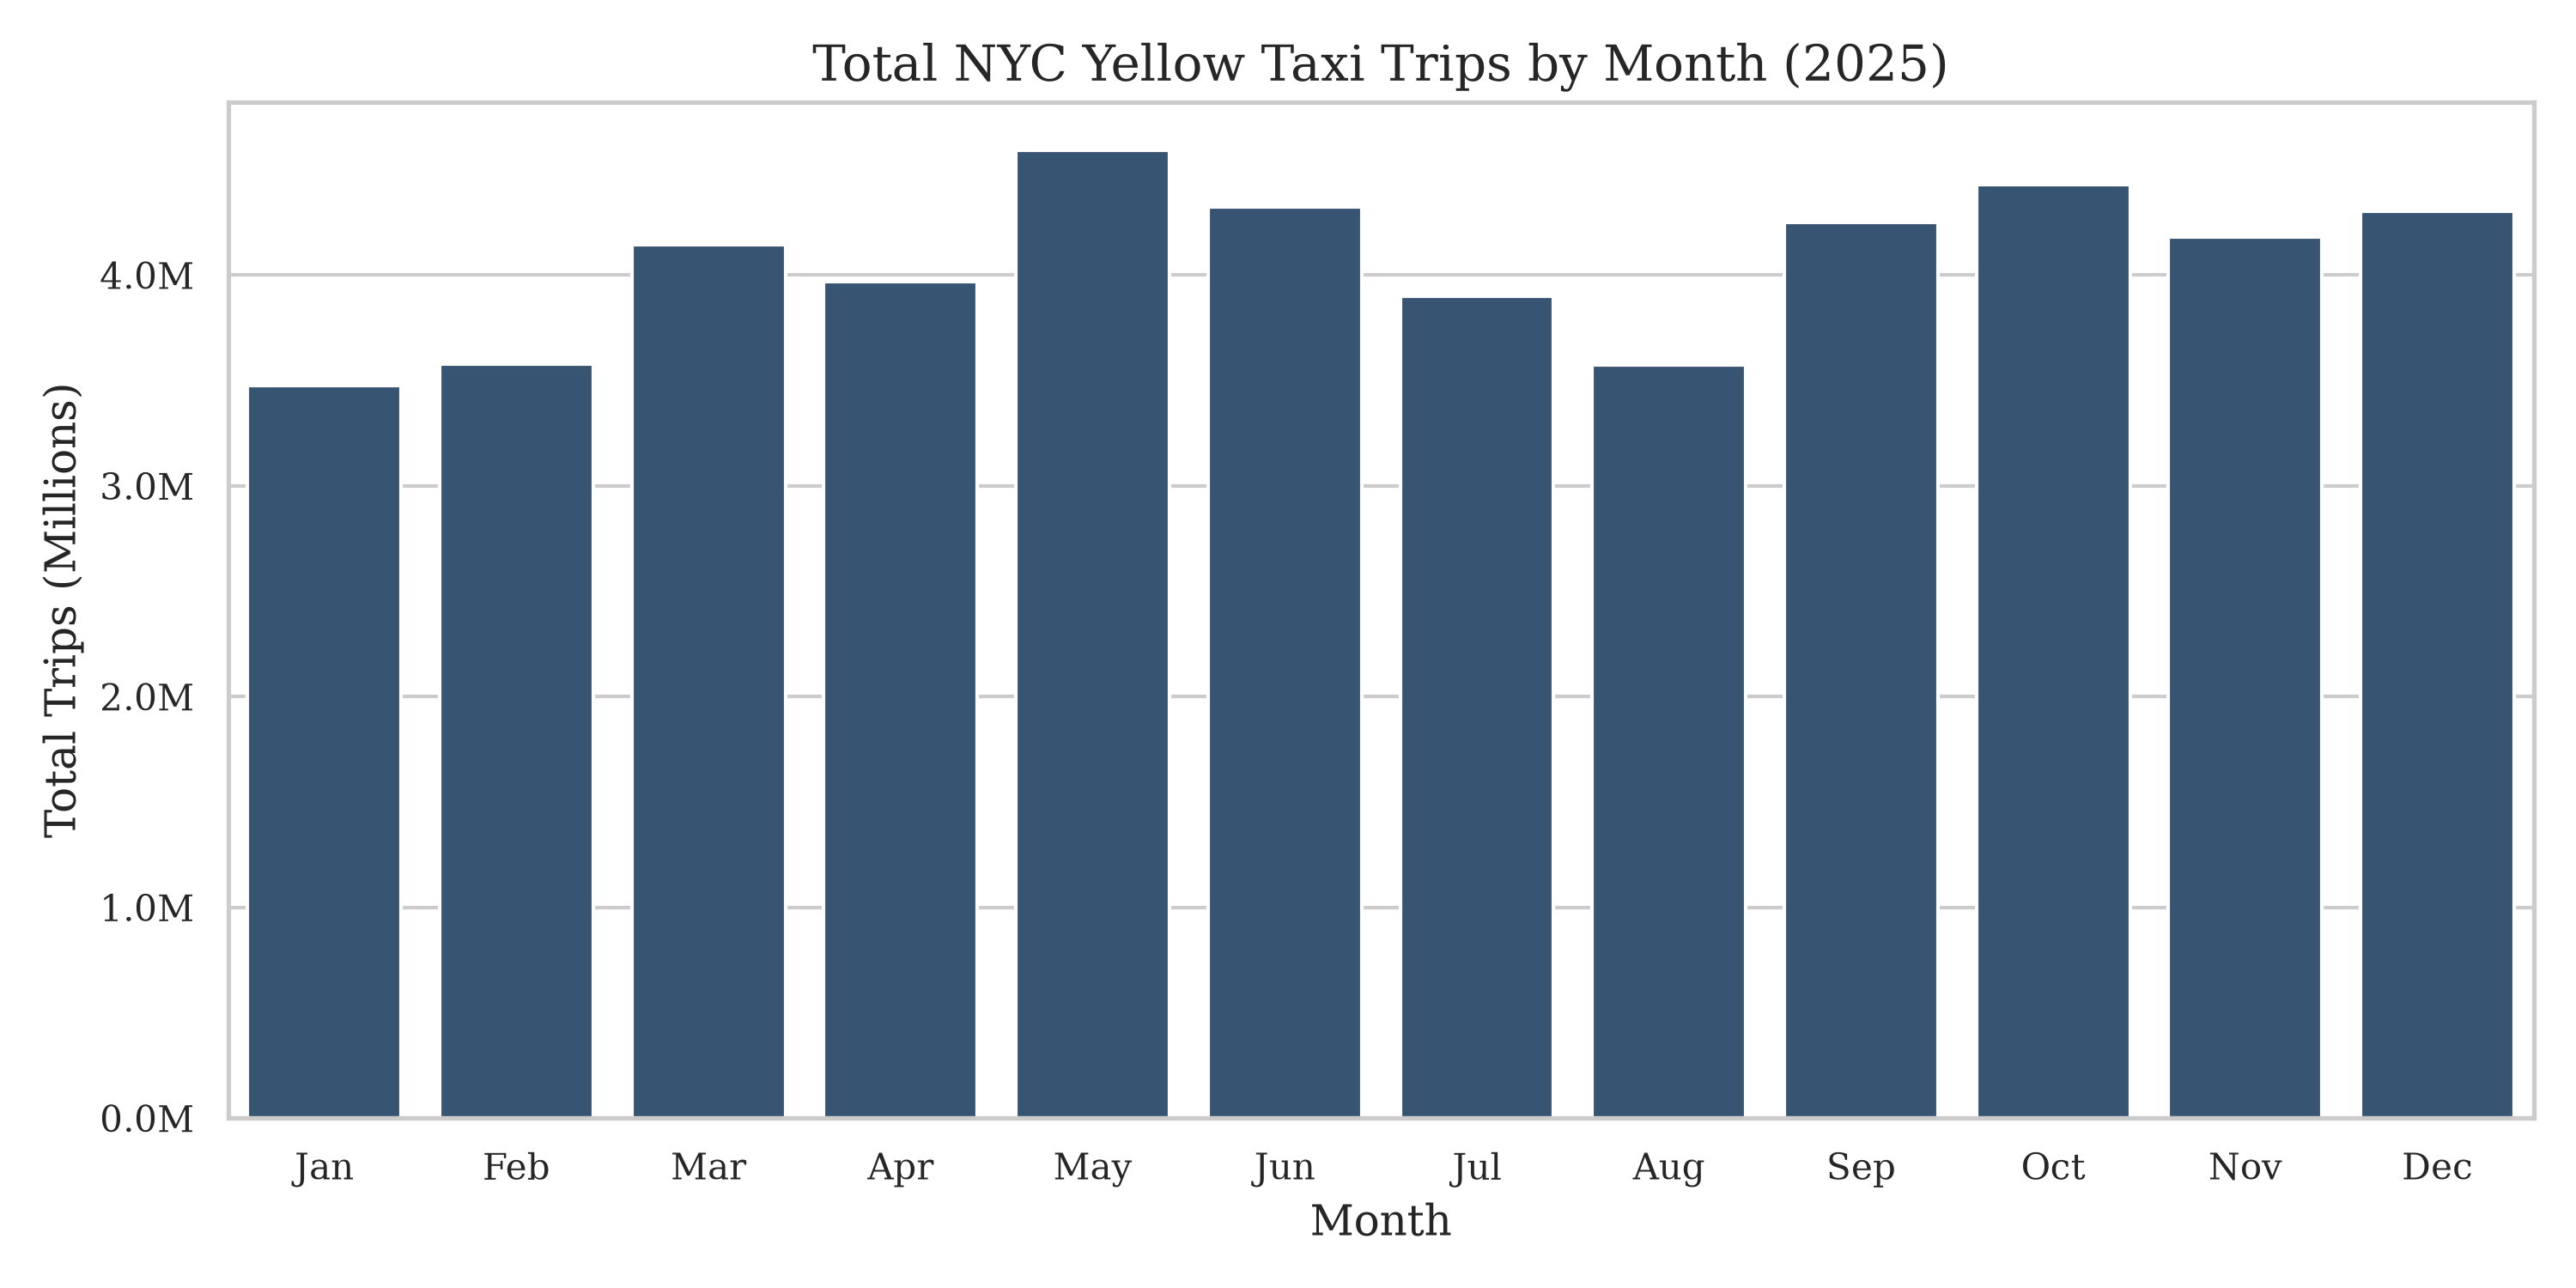
\includegraphics[width=\textwidth]{../figures/monthly_distribution.png}
        \caption{Monthly Trip Volume}
        \label{fig:monthly}
    \end{subfigure}
    \hfill
    \begin{subfigure}[b]{0.48\textwidth}
        \centering
        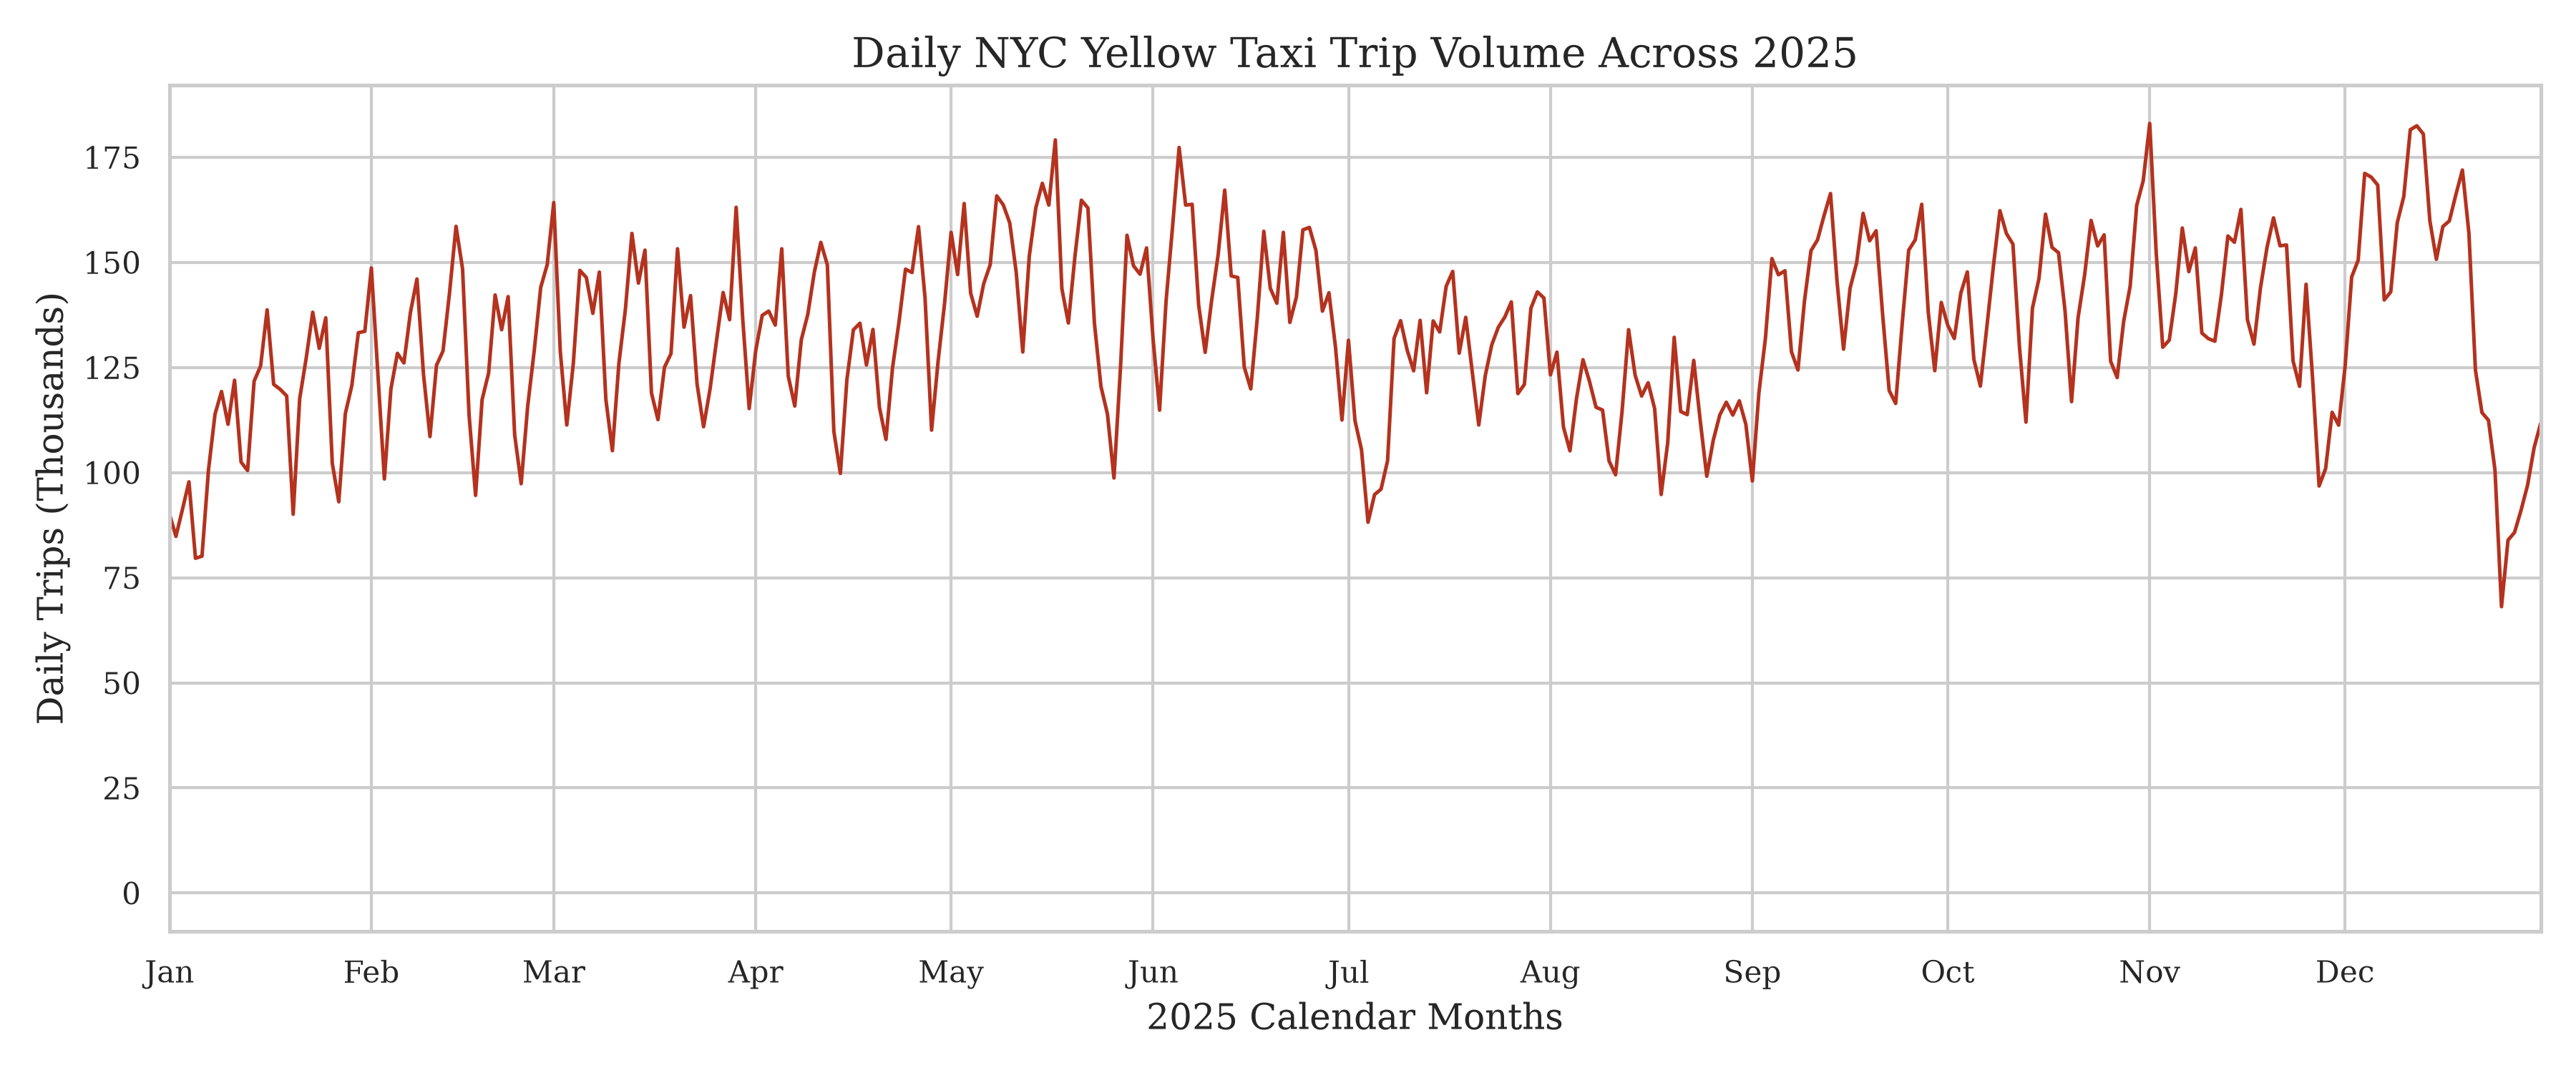
\includegraphics[width=\textwidth]{../figures/daily_timeseries.png}
        \caption{Daily Time Series}
        \label{fig:daily}
    \end{subfigure}
    
    \caption{Temporal Distribution and Time Series Analysis of NYC Yellow Taxi Trips (2025)}
    \label{fig:temporal_grid}
\end{figure}

\begin{itemize}
    \item \textbf{Intra-Day Hourly Patterns:}
     Trip volumes follow a distinct bimodal commuter curve (Figure~\ref{fig:hourly}). Activity hits its nightly trough between 03:00 and 05:00 AM ($\approx 0.35\text{M}$ trips), ramps up steadily through the morning, and peaks sharply during the evening rush hour at 18:00 (6:00 PM) with nearly $3.5\text{M}$ annual originations.
    \item 
    \textbf{Inter-Day Weekly Patterns:} 

    Weekly activity (Figure~\ref{fig:dow}) remains robust from Tuesday through Saturday, with Saturday recording the highest aggregate volume ($\approx 7.5\text{M}$ trips), driven by weekend entertainment and nightlife mobility. Monday experiences a relative weekly lull ($\approx 5.9\text{M}$ trips).
    
    \item \textbf{Monthly \& Longitudinal Trends:} 
    Monthly aggregation (Figure~\ref{fig:monthly}) highlights peak seasonal volume in May ($\approx 4.6\text{M}$ trips), while the daily time-series trend across all 365 calendar days of 2025 (Figure~\ref{fig:daily}) confirms complete temporal data continuity with zero missing daily partitions and consistent weekly oscillations.
\end{itemize}



\subsection{Exploratory Data Analysis: Trip Distance}
\label{sec:eda_trip_distance}

The \texttt{trip\_distance} variable measures the elapsed trip distance in miles as reported by the taximeter. Across the filtered 2025 dataset comprising $44,186,099$ valid trips, the distribution exhibits characteristics typical of urban high-density taxi operations.

\begin{table}[htbp]
\centering
\caption{Descriptive Statistics for Trip Distance (2025 Dataset)}
\label{tab:stats_trip_distance}
\begin{tabular}{lr}
\toprule
\textbf{Metric} & \textbf{Value} \\
\midrule
Total Valid Trips & 44,041,005 \\
Mean ($\mu$) & 3.49 miles \\
25th Percentile ($Q_1$) & 1.1 \\
Median ($Q_2$) & 1.89 miles \\
75th Percentile ($Q_3$) & 3.73 \\
Standard Deviation ($\sigma$) & 4.32 miles \\
Interquartile Range (IQR) & 2.63 miles \\
Skewness & 2.95 \\
\bottomrule
\end{tabular}
\end{table}

\subsubsection{Statistical Characteristics and Shape}
As detailed in Table~\ref{tab:stats_trip_distance}, the median trip distance is $1.89$ miles, whereas the mean is higher at $3.49$ miles. This divergence, coupled with a positive skewness of $2.95$, reflects right-skewed distribution. The probability density function (Figure~\ref{fig:trip_distance_dist}) shows a sharp concentration of mass at short distances ($<3$ miles), representing typical intra-Manhattan street hails, followed by an extended, long positive tail corresponding to regional and airport transfers.

\begin{figure}[htbp]
    \centering
    \begin{subfigure}[b]{0.48\textwidth}
        \centering
        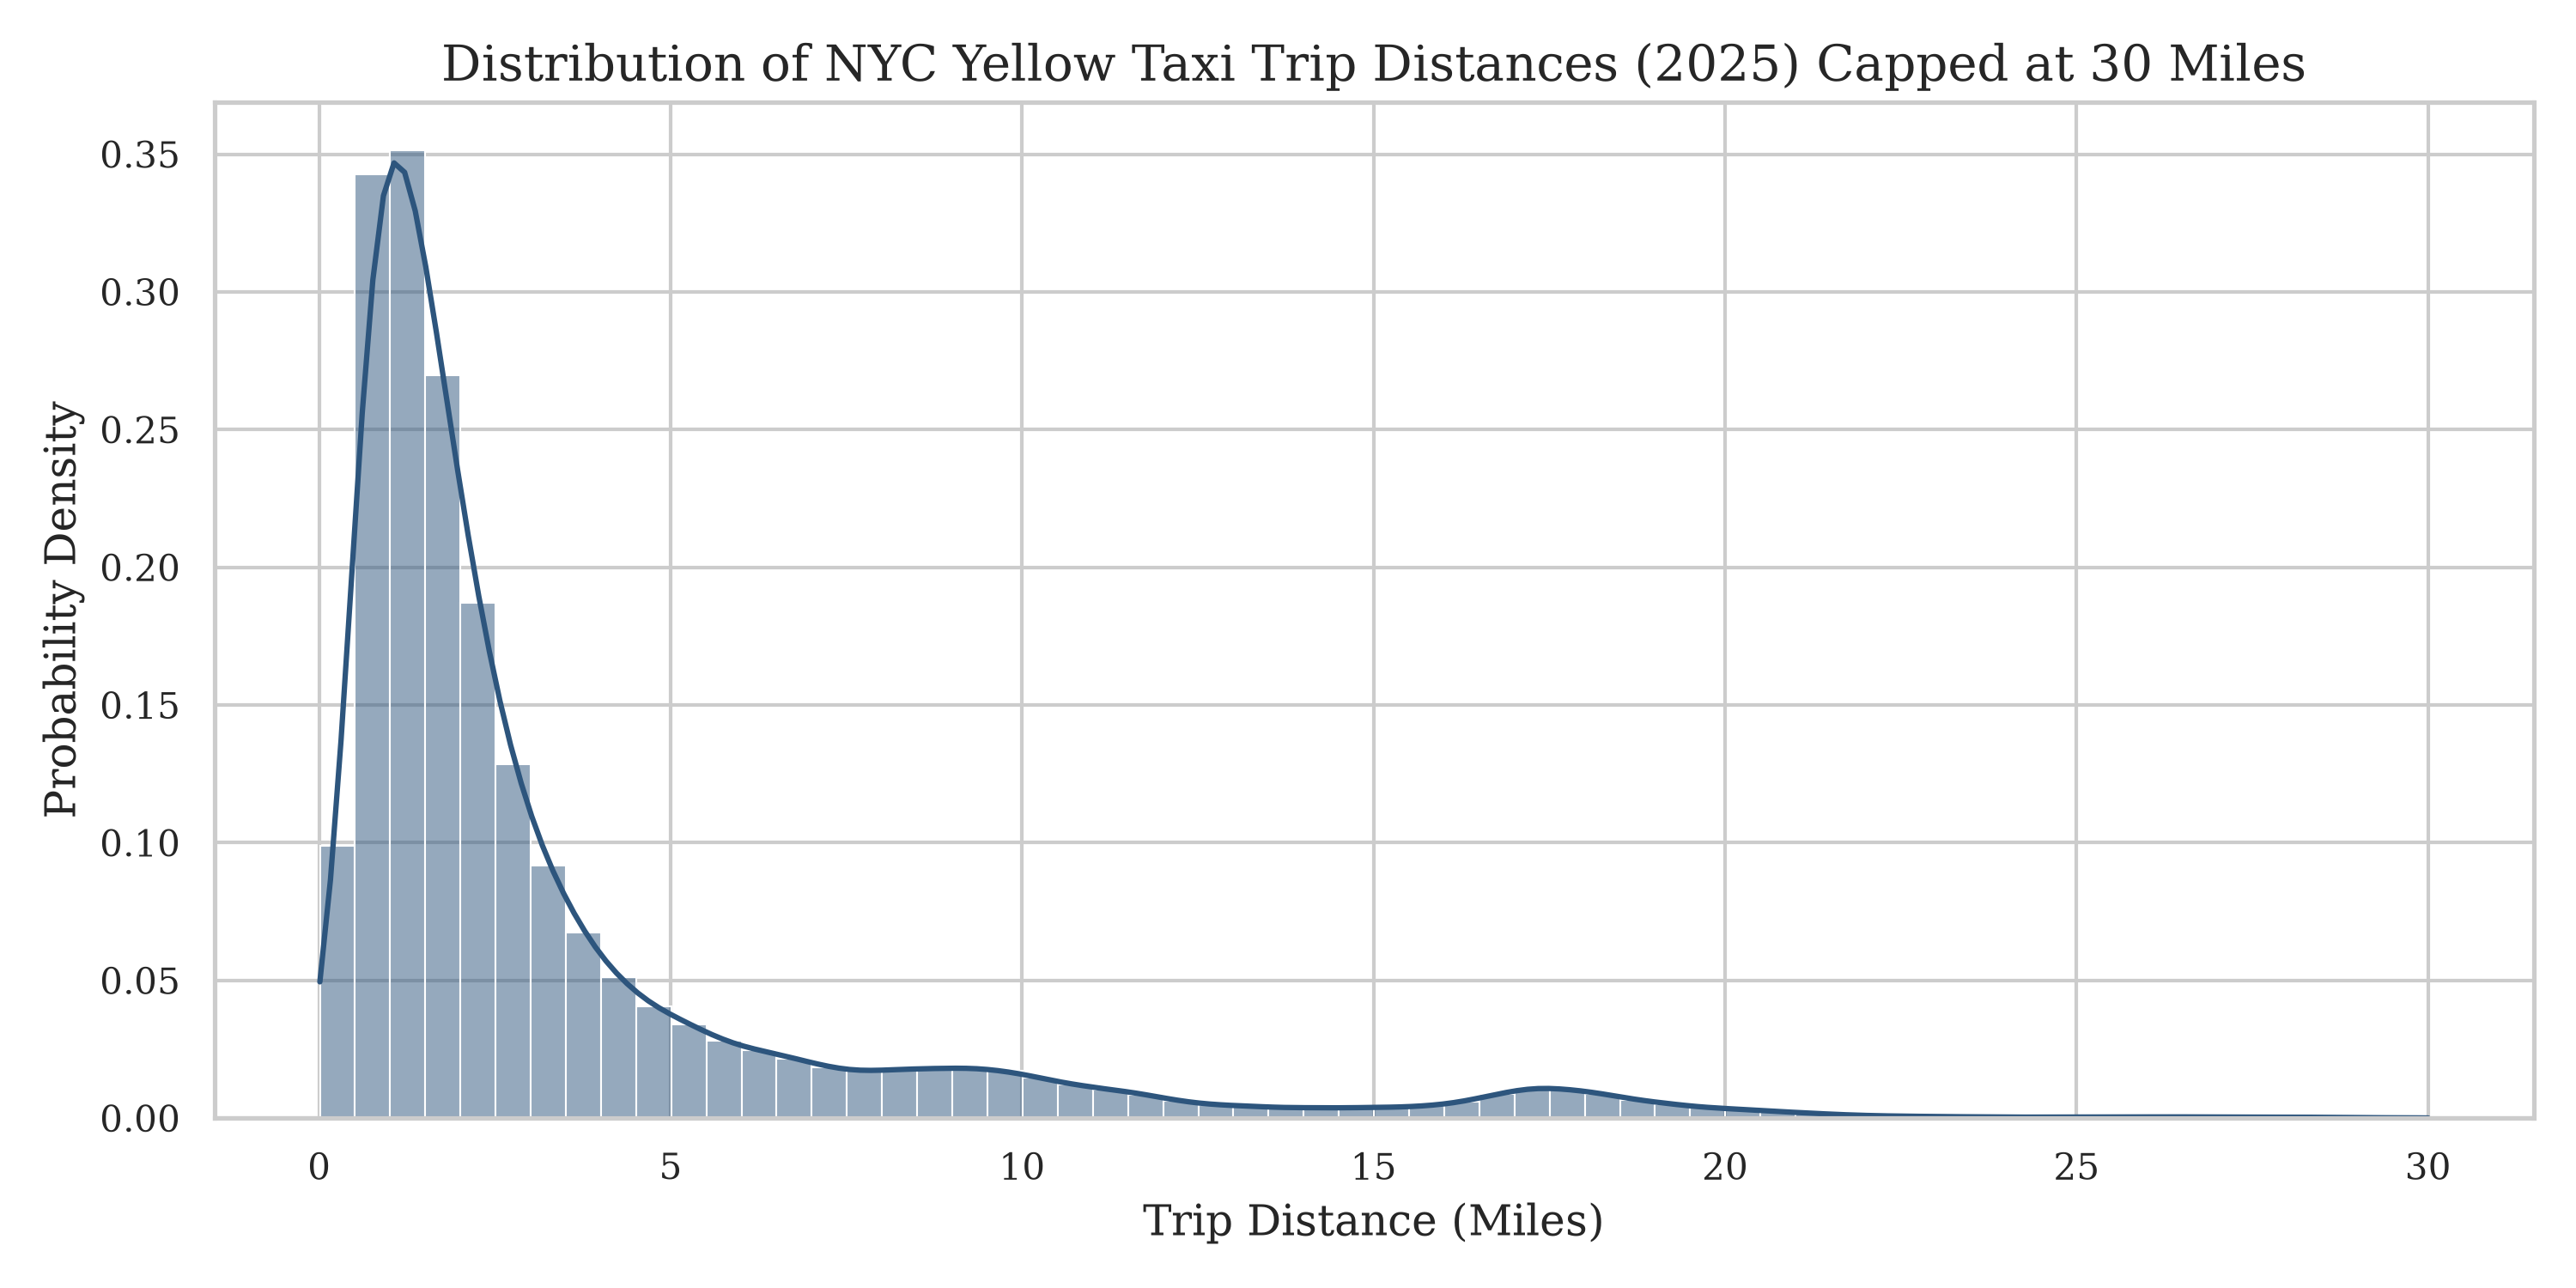
\includegraphics[width=\textwidth]{../figures/trip_distance_distribution.png}
        \caption{Probability Density Distribution Capped at 30 Miles}
        \label{fig:trip_distance_dist}
    \end{subfigure}
    \hfill
    \begin{subfigure}[b]{0.48\textwidth}
        \centering
        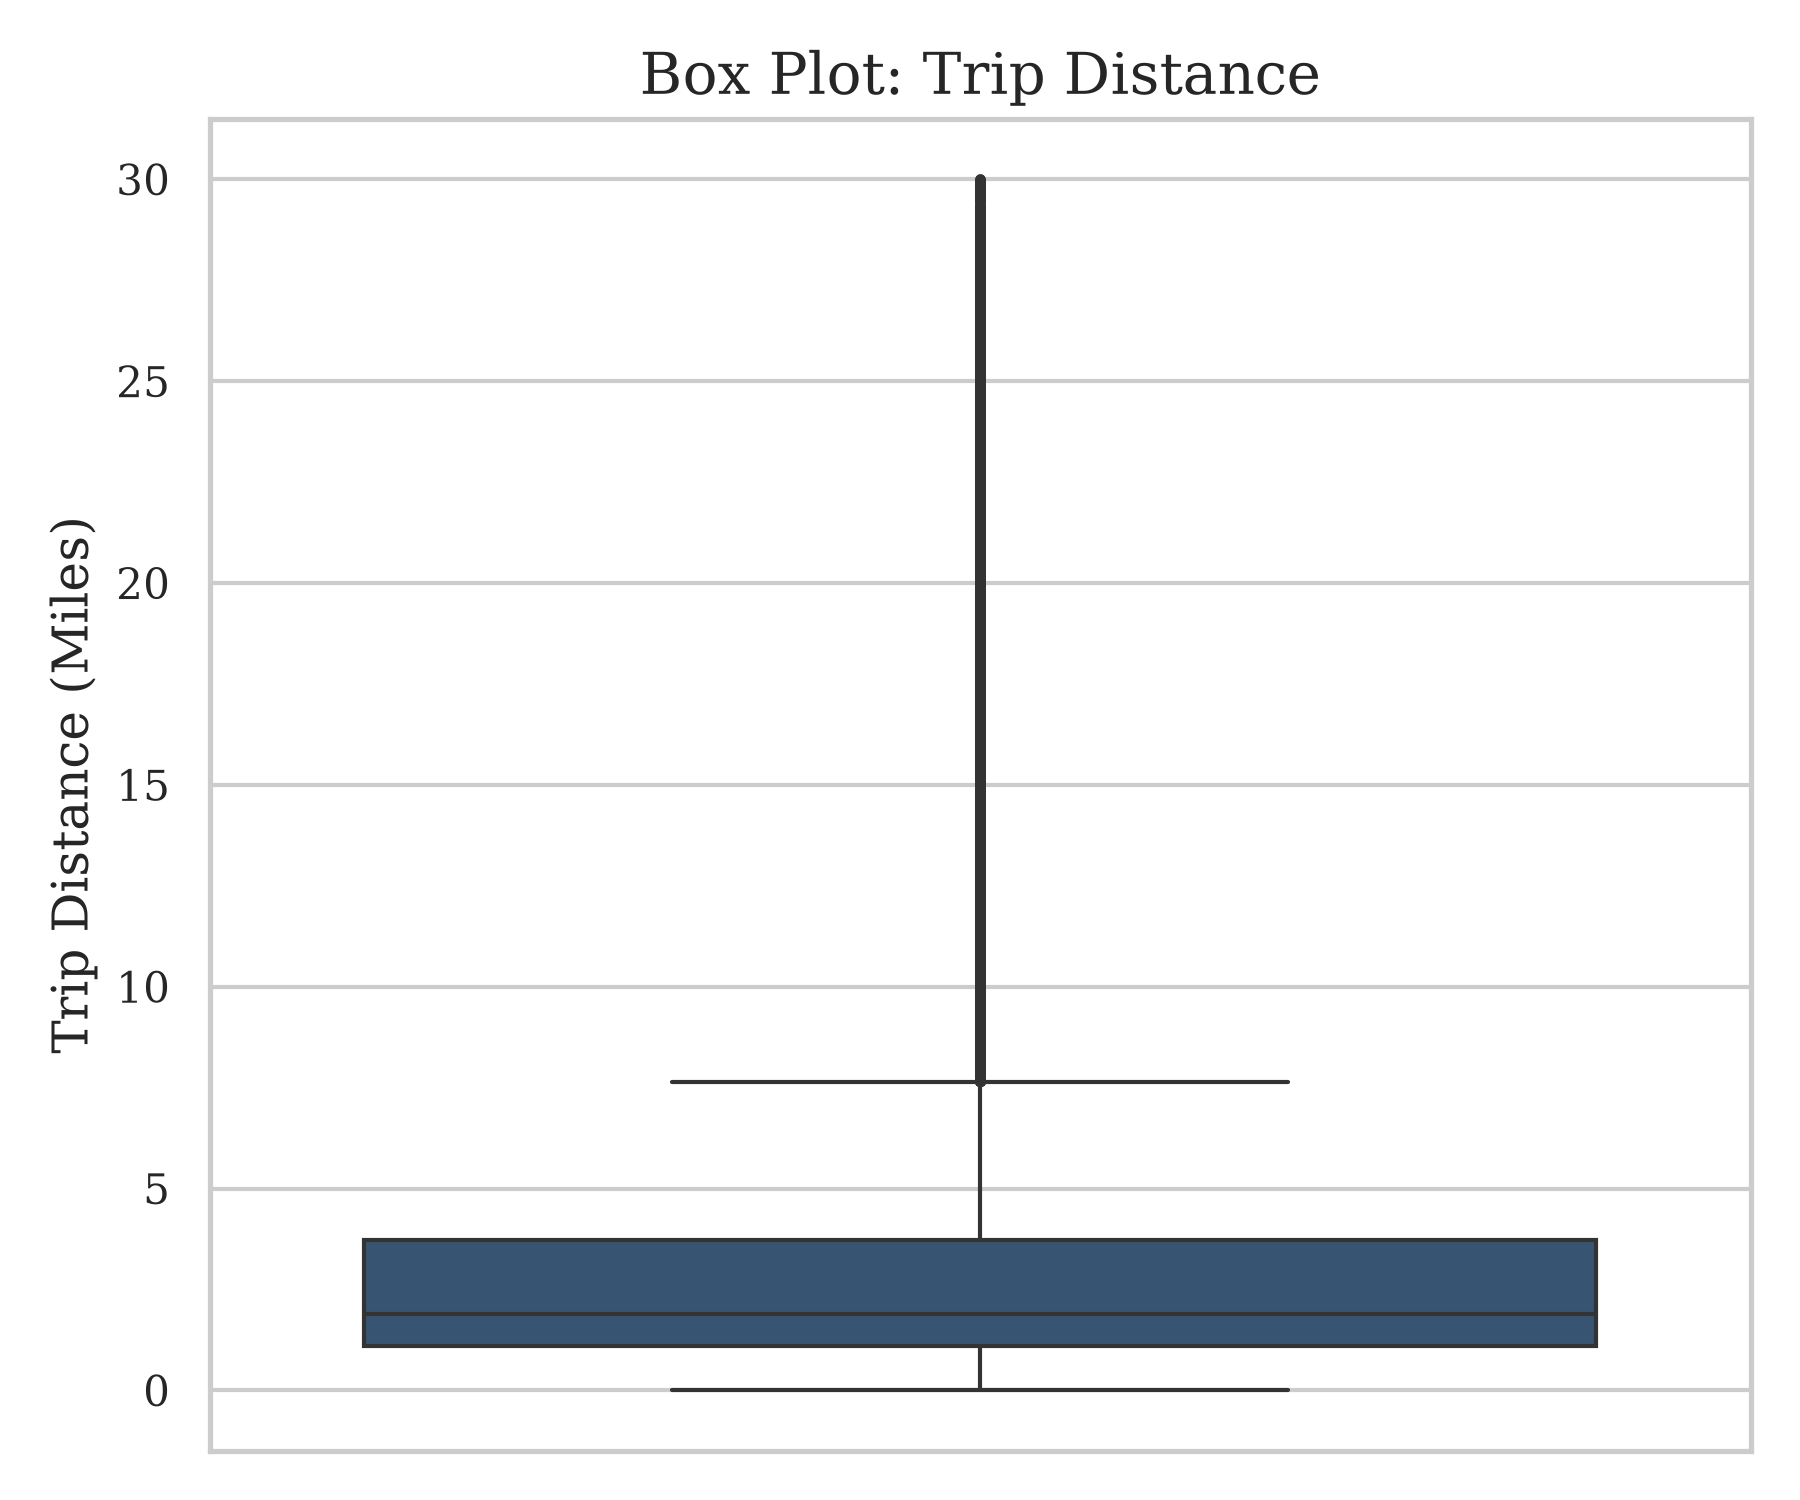
\includegraphics[width=\textwidth]{../figures/trip_distance_boxplot.png}
        \caption{Box Plot (Capped at 30 Miles)}
        \label{fig:trip_distance_box}
    \end{subfigure}
    \caption{Distribution and Box Plot Analysis for Trip Distance (2025)}
    \label{fig:trip_distance_analysis}
\end{figure}

\subsubsection{Long-Distance Trips and Outlier Analysis ($>30$ Miles)}

A detailed query of trips exceeding $30$ miles yields a total of \textbf{41,581 valid long-distance trips} across the 2025 dataset ($\approx 0.095\%$ of all clean trips). Table~\ref{tab:long_distance_trips} illustrates a representative sample of these extreme-distance records, ordered by descending distance.

\begin{table}[htbp]
\centering
\caption{Sample of Long-Distance Yellow Taxi Trips Exceeding 30 Miles (2025)}
\label{tab:long_distance_trips}
\small
\begin{tabularx}{\textwidth}{llrrlXX}
\toprule
\textbf{Pickup Time} & \textbf{Dropoff Time} & \textbf{Pass.} & \textbf{Dist. (mi)} & \textbf{Fare (\$)} & \textbf{Pickup Zone} & \textbf{Dropoff Zone} \\
\midrule
2025-05-31 10:28 & 2025-05-31 12:33 & 1 & 99.82 & \$105.90 & South Ozone Park & Outside of NYC \\
2025-11-21 12:00 & 2025-11-21 14:21 & 2 & 99.81 & \$200.00 & Clinton East & Outside of NYC \\
2025-06-05 16:40 & 2025-06-05 19:15 & 1 & 99.80 & \$358.60 & JFK Airport & Outside of NYC \\
2025-10-12 21:57 & 2025-10-13 01:28 & 1 & 99.80 & \$122.00 & Springfield Gardens South & Bay Ridge \\
2025-07-04 21:04 & 2025-07-04 22:49 & 1 & 99.73 & \$637.90 & Penn Station/Madison Sq West & Outside of NYC \\
2025-12-27 09:45 & 2025-12-27 11:38 & N/A & 99.70 & \$346.57 & Midtown Center & Outside of NYC \\
2025-02-17 19:51 & 2025-02-17 21:50 & 2 & 99.68 & \$230.00 & West Village & Outside of NYC \\
2025-08-12 13:25 & 2025-08-12 15:24 & 1 & 99.54 & \$670.80 & JFK Airport & Outside of NYC \\
2025-08-20 07:10 & 2025-08-20 09:47 & 1 & 99.46 & \$350.00 & JFK Airport & Outside of NYC \\
2025-12-23 07:31 & 2025-12-23 12:23 & 1 & 99.46 & \$650.50 & JFK Airport & Outside of NYC \\
\bottomrule
\end{tabularx}
\end{table}

\subsubsection{Justification for Retaining Outliers Beyond the 1.5$\times$IQR Rule}
In standard exploratory data analysis, Tukey's fence rule classifies any observation exceeding $Q_3 + 1.5 \times \text{IQR}$ as an outlier. Given $Q_3 = 4.52$ miles and an IQR of $2.63$ miles, this traditional threshold flags any trip longer than approximately $8.465$ miles as an outlier candidate for deletion. 

However, \textbf{these extreme values are strictly retained rather than trimmed} for the following operational and empirical reasons:
\begin{enumerate}
    \item \textbf{Legitimate Out-of-Jurisdiction and Regional Transit Activity:} As demonstrated in Table~\ref{tab:long_distance_trips}, the majority of extreme long-distance trips originate at major hubs (e.g., JFK Airport, Midtown Center, Penn Station) and terminate at \texttt{Outside of NYC} destinations (e.g., Westchester, Long Island, New Jersey, or Upstate New York). These represent $41,581$ legitimate, highly profitable commercial journeys that taxi drivers are legally contracted to fulfill.
    \item \textbf{Economic Integrity and Revenue Preservation:} Removing trips beyond $8.465$ miles would wipe out a substantial portion of total fare volume and artificially distort demand models. Out-of-city and airport transit runs account for premium fares (ranging up to \$670.80 in our sample) and contribute significantly to gross fleet earnings and total congestion surcharge revenues.
    \item \textbf{Prevention of Truncation Bias in Spatial Aggregation:} Artificially capping or trimming distance values would corrupt origin-destination flow matrices and underestimate vehicle turnover and idle times required for long-distance returns.
    \item \textbf{Methodological Handling over Destructive Trimming:} Rather than dropping valid data, we accommodate extreme skewness ($\text{Skewness} = 254.71$) through non-parametric location measures (median $= 1.89$ miles, IQR $= 2.63$ miles) and visual capping (e.g., truncating axes at $30$ miles in distribution plots) to maintain graphic clarity while preserving $100\%$ of underlying economic activity.
\end{enumerate}


\subsection{Exploratory Data Analysis: Fare Amount}
\label{sec:eda_fare_amount}

The \texttt{fare\_amount} variable represents the time-and-distance fare in USD calculated by the taximeter at the conclusion of each trip. Across the processed 2025 dataset comprising $44,041,005$ valid records, fare pricing reflects standard urban meter tariffs combined with regulatory flat-rate structures.

\begin{table}[htbp]
\centering
\caption{Descriptive Statistics for Fare Amount (2025 Dataset)}
\label{tab:stats_fare_amount}
\begin{tabular}{lr}
\toprule
\textbf{Metric} & \textbf{Value} \\
\midrule
Total Valid Trips & 44,041,005 \\
Mean ($\mu$) & \$20.04 \\
25th Percentile ($Q_1$) & \$9.3 \\
Median ($Q_2$) & \$14.20 \\
75th Percentile ($Q_3$) & \$23.3 \\
Standard Deviation ($\sigma$) & \$149.70 \\
Interquartile Range (IQR) & \$14.00 \\
Skewness & 4834.15 \\
\bottomrule
\end{tabular}
\end{table}

\subsubsection{Statistical Characteristics and Shape}
As summarized in Table~\ref{tab:stats_fare_amount}, the median fare is $\$14.20$, while the mean is higher at $\$20.04$. The distribution exhibits extreme positive skewness ($4834.15$), driven by a heavy concentration of short, low-cost urban trips and an extended right-hand tail of high-value journeys. 

The probability density function (Figure~\ref{fig:fare_amount_dist}) reveals a prominent unimodal peak representing standard local city rides ($\$10-\$15$), alongside a distinct structural cluster or secondary bump around $\$70$. This secondary surge corresponds directly to regulated flat-rate airport trips (such as historical or standard JFK airport routes), highlighting a multimodal element embedded within the financial structure of the fleet.

\begin{figure}[htbp]
    \centering
    \begin{minipage}[b]{0.48\textwidth}
        \centering
        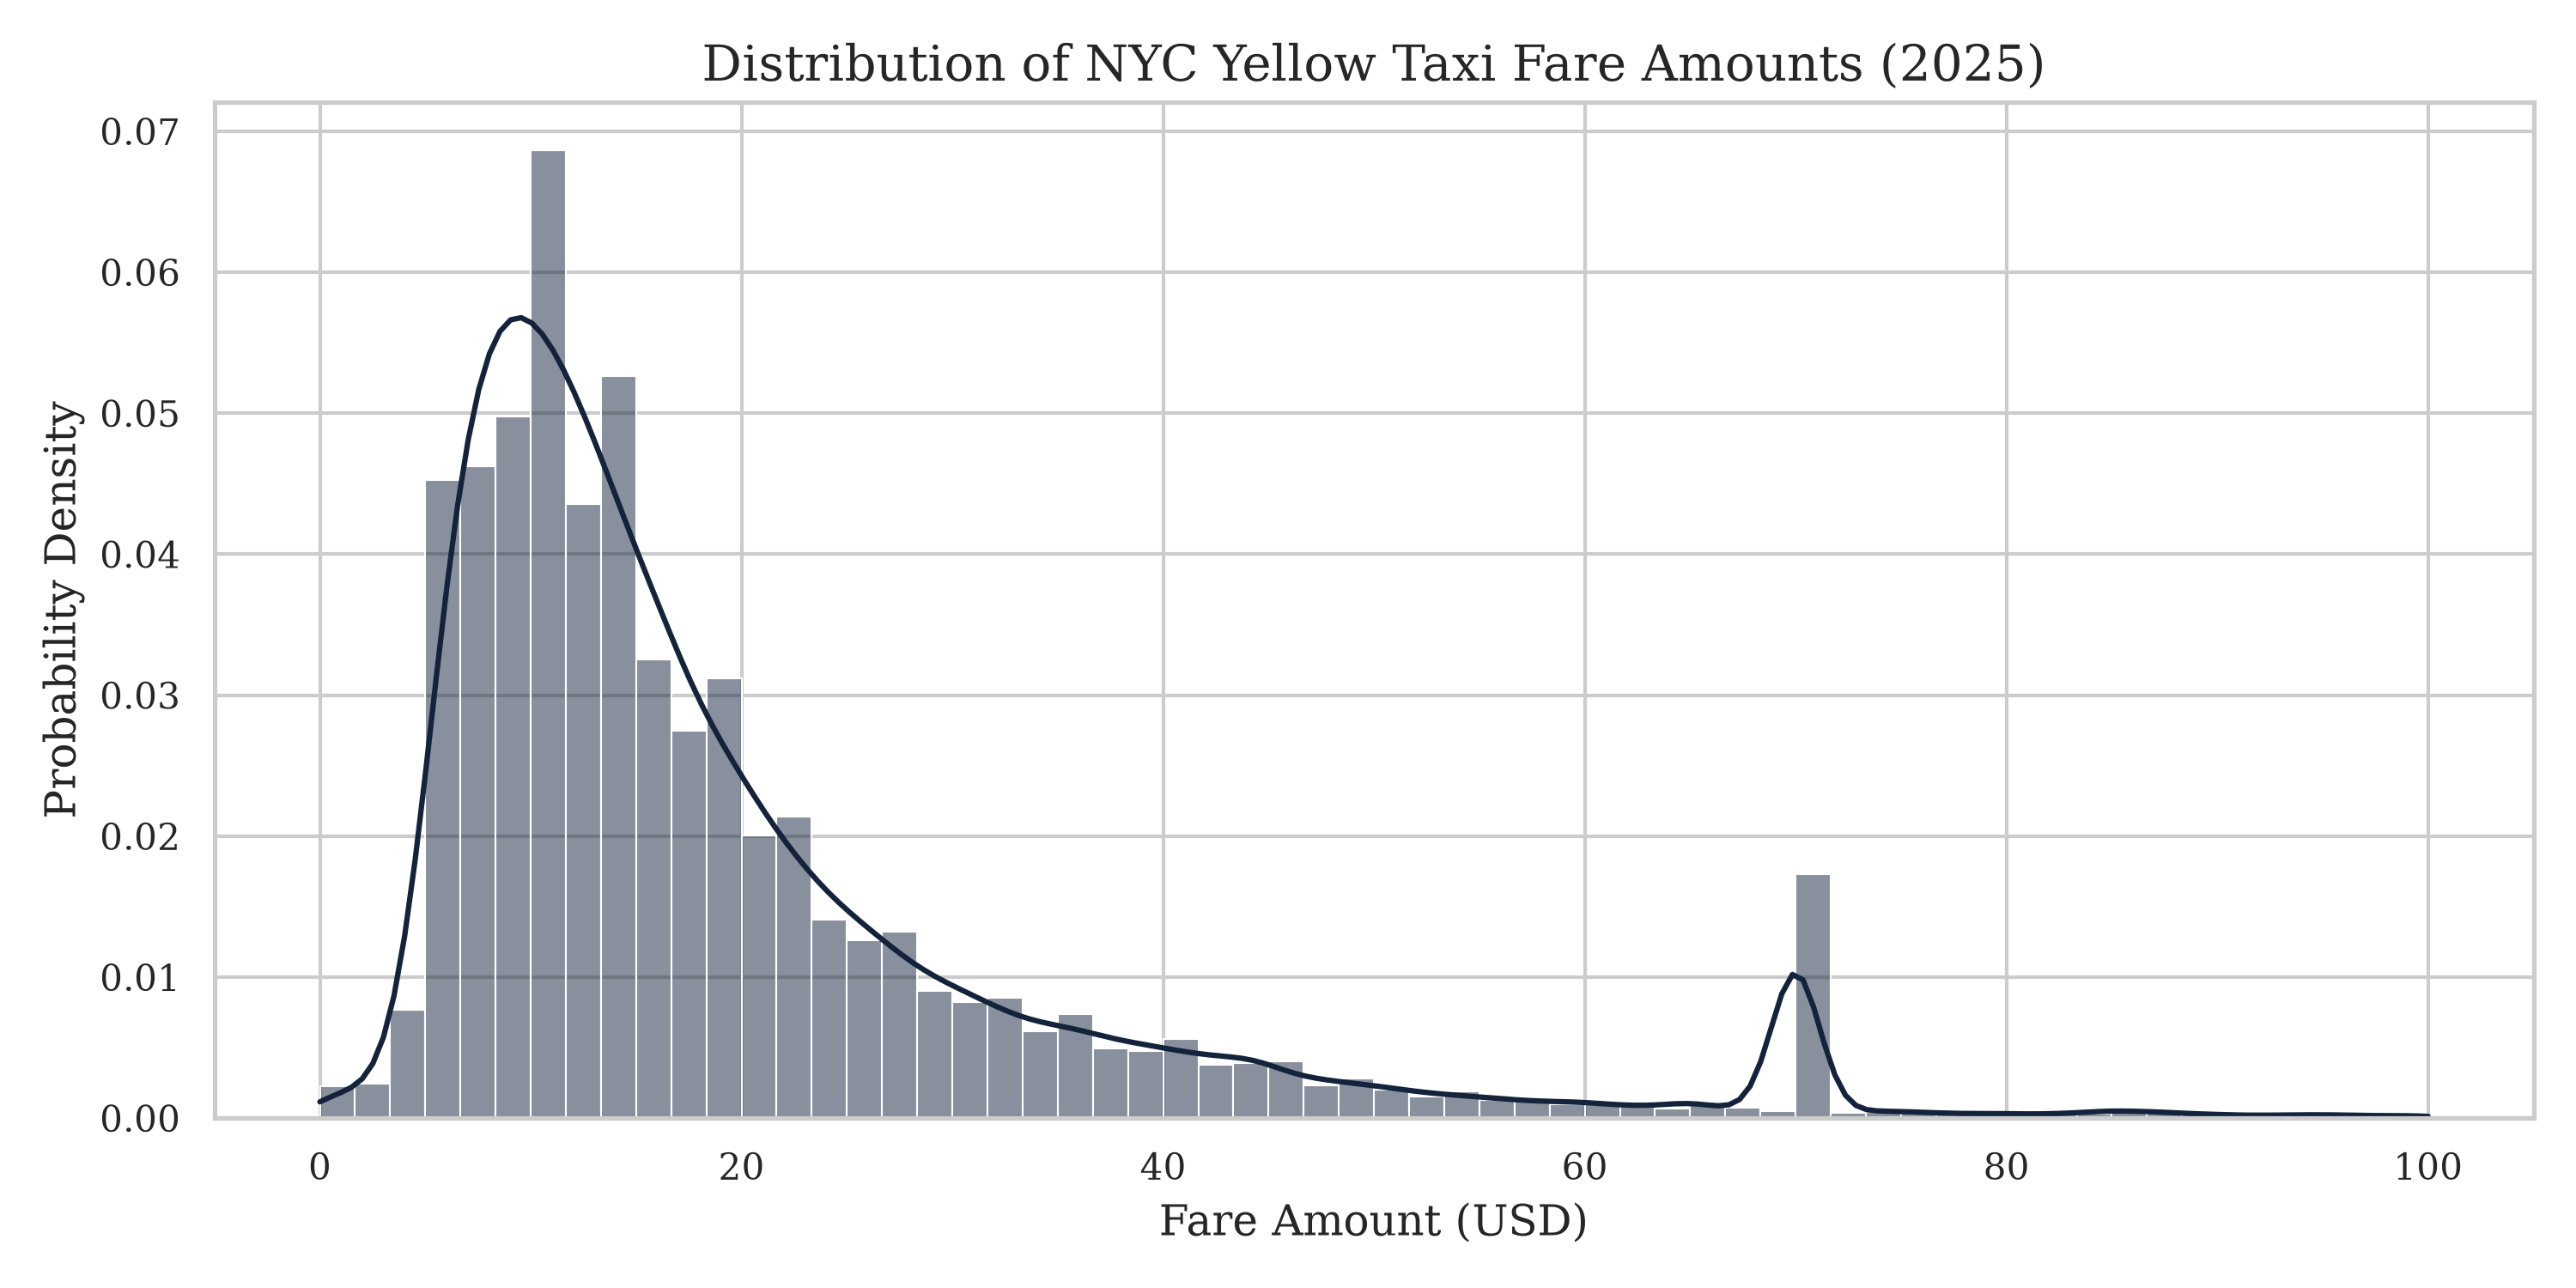
\includegraphics[width=\textwidth]{../figures/fare_amount_distribution.png}
        \caption{Probability Density Distribution}
        \label{fig:fare_amount_dist}
    \end{minipage}
    \hfill
    \begin{minipage}[b]{0.48\textwidth}
        \centering
        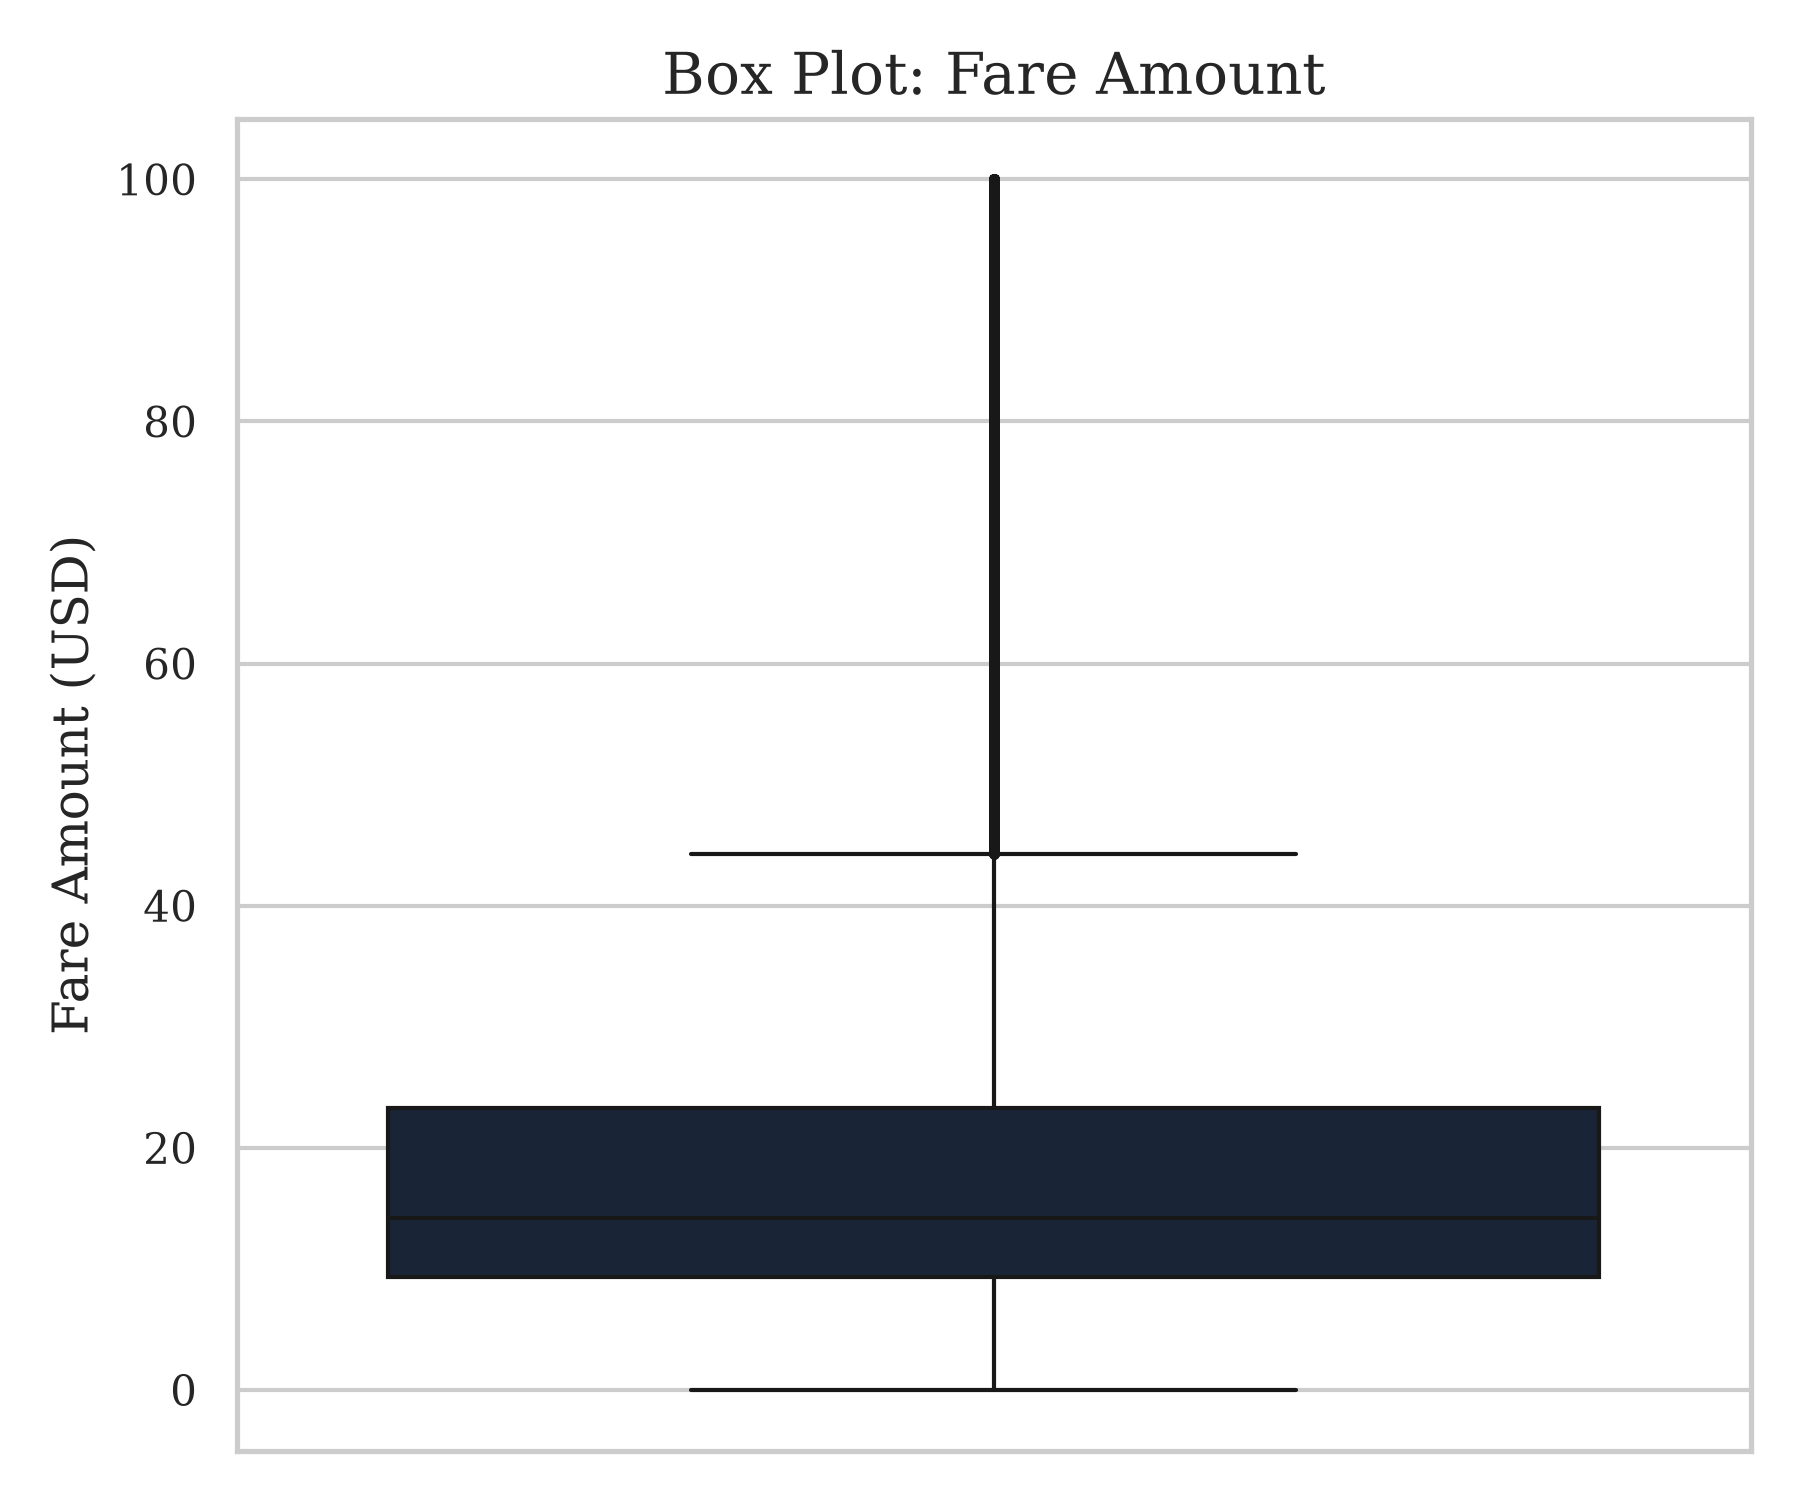
\includegraphics[width=\textwidth]{../figures/fare_amount_boxplot.png}
        \caption{Box Plot (Capped at \$100)}
        \label{fig:fare_amount_box}
    \end{minipage}
    \caption{Distribution and Box Plot Analysis for Fare Amount (2025)}
    \label{fig:fare_amount_analysis}
\end{figure}

\subsubsection{Justification for Retaining Outliers Beyond the 1.5$\times$IQR Rule}
Under standard Tukey fence criteria, the upper bound for outliers is defined as $Q_3 + 1.5 \times \text{IQR}$. Given an approximate third quartile $Q_3 = \$23.30$ and an IQR of $\$14.00$, this traditional threshold flags any fare exceeding approximately $\$44.30$ as an outlier.

However, \textbf{these high-value fare observations are strictly retained rather than trimmed} for the following operational and economic reasons:
\begin{enumerate}
    \item \textbf{Commercial Validity of Airport Flat Rates:} Fares exceeding the $\$42.20$ threshold are not data errors or anomalies; they represent authorized high-value commercial transactions, most notably the regulated flat rates for trips between Manhattan and major regional airports ($\approx \$70$, clearly visible in Figure~\ref{fig:fare_amount_dist}). Deleting these records would discard crucial airport demand data.
    \item \textbf{Prevention of Economic Distortion:} Trimming observations beyond the $1.5 \times \text{IQR}$ fence would artificially deflate total revenue estimates, average ticket sizes, and macro-economic metrics across the dataset. Retaining them preserves the true economic distribution of NYC yellow taxi operations.
    \item \textbf{Robust Analytical Presentation:} Rather than destructive data filtering, extreme financial values are managed through robust location-and-spread metrics (median and IQR) and visual capping (\$100 ceiling in Figure~\ref{fig:fare_amount_box}) to ensure graphical readability while maintaining complete data fidelity.
\end{enumerate}

\subsection{Exploratory Data Analysis: Central Business District Congestion Fee}
\label{sec:eda_cbd_congestion_fee}

The \texttt{cbd\_congestion\_fee} variable captures the Central Business District (CBD) congestion toll structure introduced across Manhattan's commercial core. Across the $44,186,099$ valid trips evaluated in the 2025 dataset, this feature reflects discrete regulatory pricing policy implementations rather than continuous meter charges.

\begin{table}[htbp]
\centering
\caption{Descriptive Statistics for CBD Congestion Fee (2025 Dataset)}
\label{tab:stats_cbd_congestion_fee}
\begin{tabular}{lr}
\toprule
\textbf{Metric} & \textbf{Value} \\
\midrule
Total Valid Trips & 44,041,005   \\
Mean ($\mu$) & \$0.55 \\
25th Percentile ($Q_1$) & 0.0 \\
Median ($Q_2$) & \$0.75 \\
75th Percentile ($Q_3$) & 0.75 \\
Standard Deviation ($\sigma$) & \$0.33 \\
Interquartile Range (IQR) & \$0.75 \\
Skewness & -1.04 \\
\bottomrule
\end{tabular}
\end{table}

\subsubsection{Statistical Characteristics and Regulatory Structure}
As detailed in Table~\ref{tab:stats_cbd_congestion_fee}, the mean fee across all recorded trips is $\$0.55$, with a median ($Q_2$) and interquartile range (IQR) of $\$0.75$. The negative skewness ($-1.04$) denotes a distribution dominated by the upper discrete fee tier.
\begin{figure}[htbp]
    \centering
    \begin{subfigure}[b]{0.48\textwidth}
        \centering
        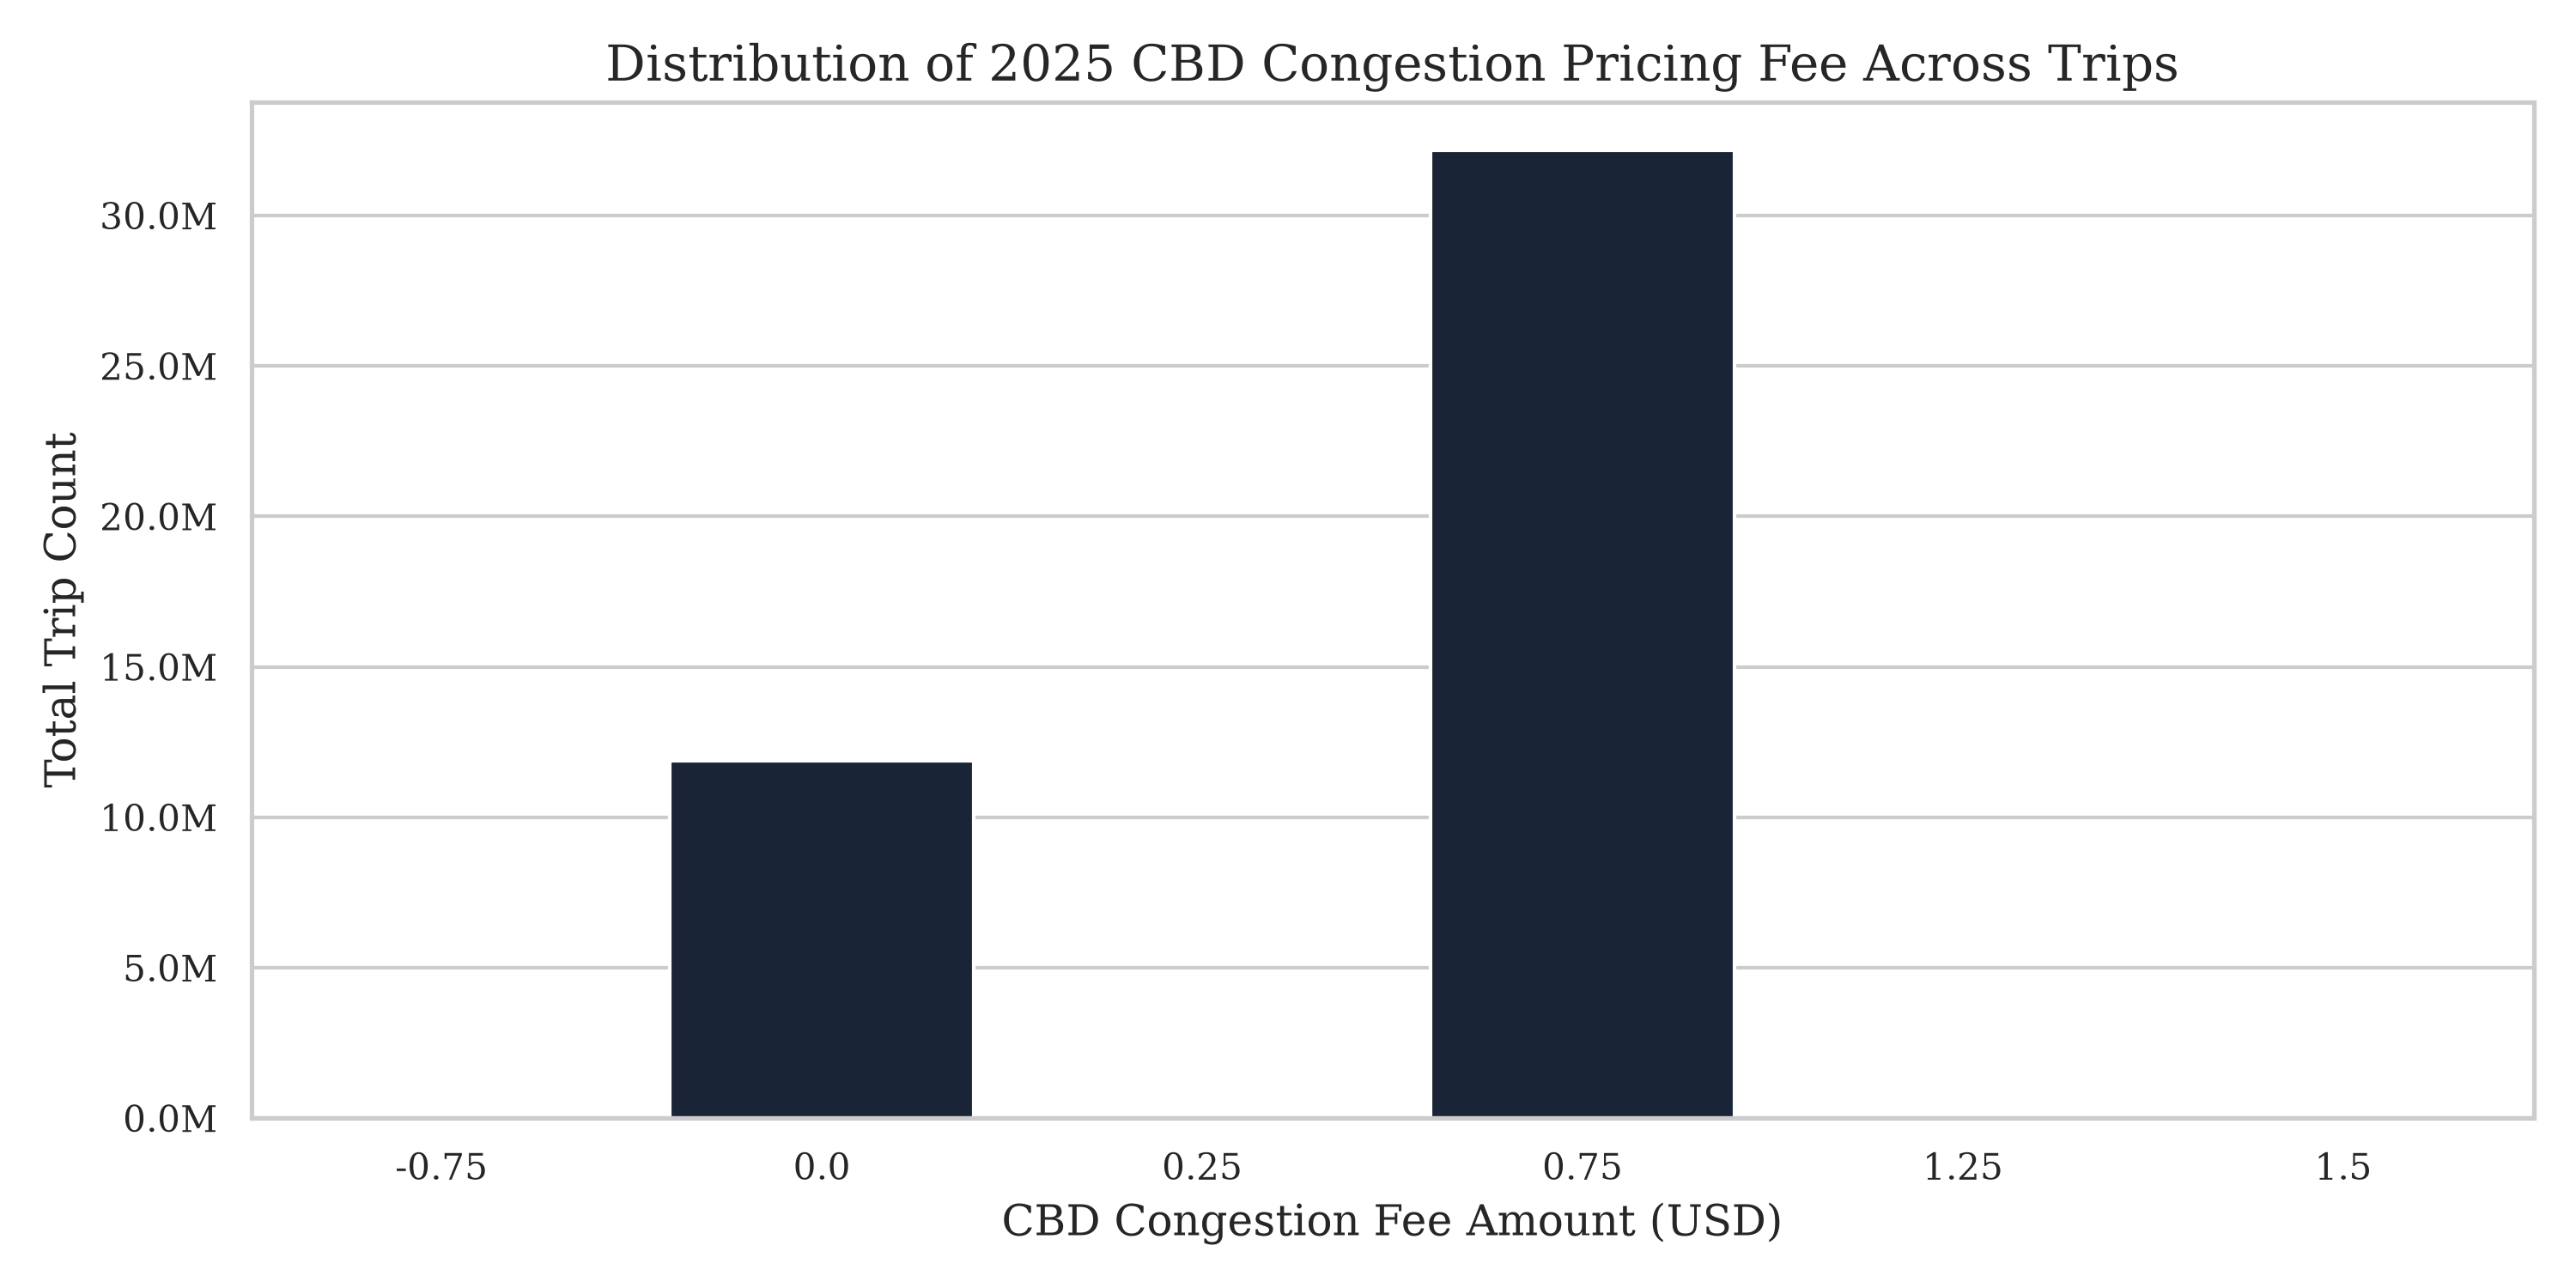
\includegraphics[width=\textwidth]{../figures/cbd_congestion_fee_distribution.png}
        \caption{Frequency Distribution across Fee Tiers}
        \label{fig:cbd_congestion_fee_dist}
    \end{subfigure}
    \hfill
    \begin{subfigure}[b]{0.48\textwidth}
        \centering
        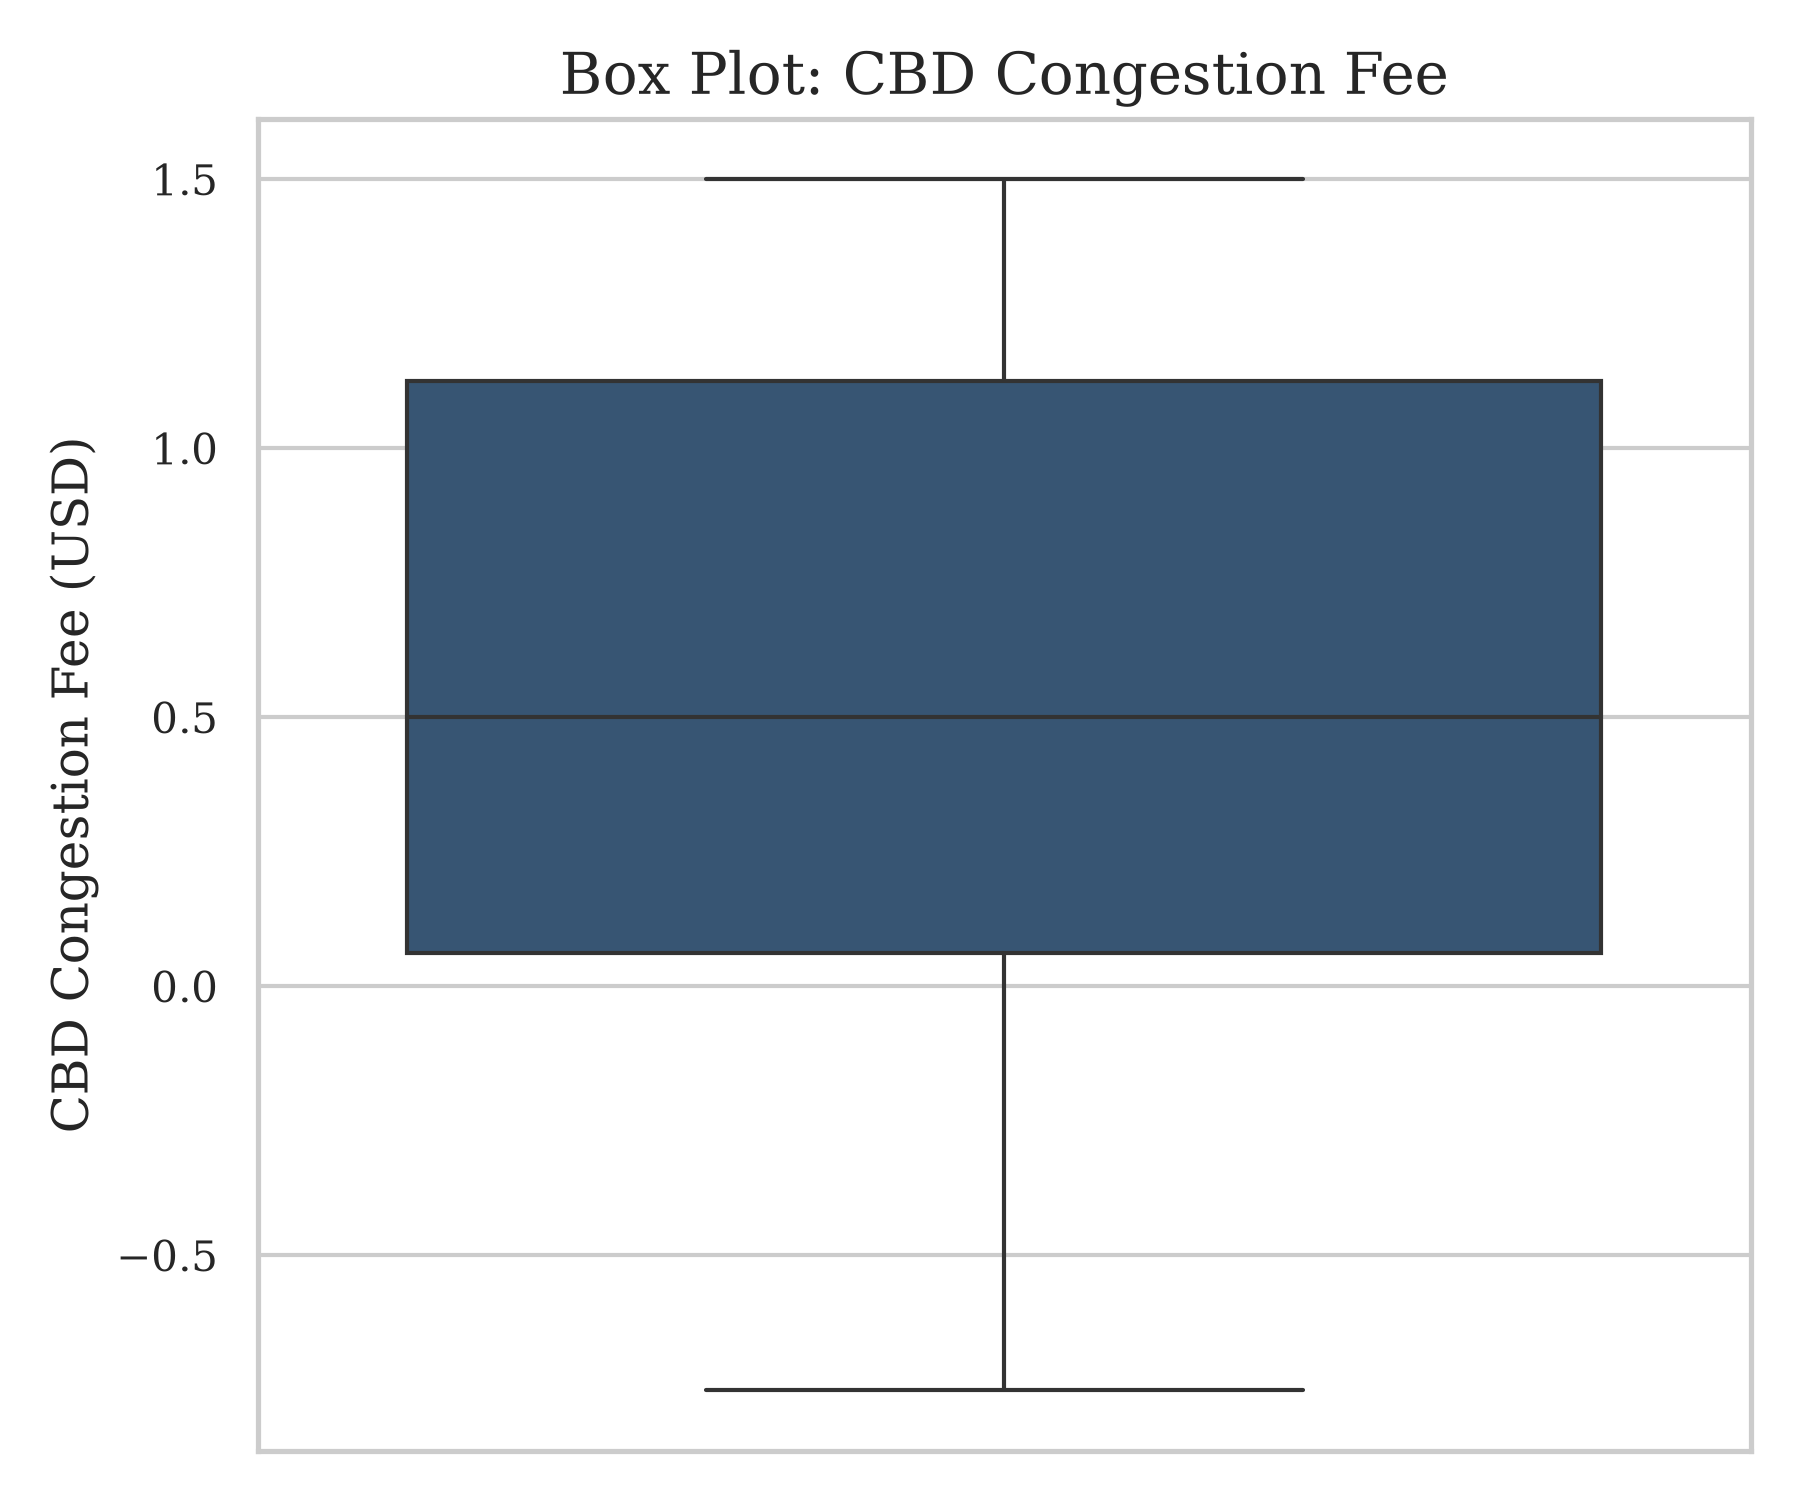
\includegraphics[width=\textwidth]{../figures/cbd_congestion_fee_boxplot.png}
        \caption{Box Plot for Discrete Policy Levels}
        \label{fig:cbd_congestion_fee_box}
    \end{subfigure}
    \caption{Distribution and Box Plot Analysis for CBD Congestion Fee (2025)}
    \label{fig:cbd_congestion_fee_analysis}
\end{figure}
Unlike continuous distance or fare measures, the fee follows a strict, highly concentrated discrete distribution (Figure~\ref{fig:cbd_congestion_fee_dist}):
\begin{enumerate}
    \item \textbf{Active Congestion Toll Tier ($\$0.75$):} Captures approximately $32$ million trips (over $72\%$ of the total fleet volume), corresponding to journeys entering, exiting, or operating entirely within the designated Manhattan CBD zone.
    \item \textbf{Exempt/Non-Zone Tier ($\$0.00$):} Accounted for by roughly $12$ million trips ($\approx 28\%$), representing outer-borough trips or movements operating outside the congestion perimeter.
\end{enumerate}

\subsubsection{Data Integrity and Analytical Interpretation}
Because \texttt{cbd\_congestion\_fee} represents a policy-mandated discrete regulatory toll, standard continuous outlier filtering methods (such as Tukey's $1.5 \times \text{IQR}$ rule) do not apply. As displayed in the box plot (Figure~\ref{fig:cbd_congestion_fee_box}), the distribution spans bounded policy levels without arbitrary extreme points. Retaining both $\$0.00$ and $\$0.75$ values is essential for evaluating fleet policy compliance, revenue collection accuracy, and spatial traffic impacts within Manhattan's core.


\subsection{Exploratory Data Analysis: Passenger Count}
\label{sec:eda_passenger_count}

The \texttt{passenger\_count} variable tracks the number of passengers reported by the driver during the trip. Across the 2025 dataset, while unrecorded or missing passenger entries account for $11,611,894$ records ($23.83\%$ of total raw volume), the subset of valid, explicitly recorded trips comprises $35,336,648$ records. Passenger occupancy patterns across this valid subset demonstrate the heavy prevalence of single-occupancy transit typical of urban yellow taxi services.

\begin{table}[htbp]
\centering
\caption{Descriptive Statistics for Valid Passenger Count (2025 Dataset)}
\label{tab:stats_passenger_count}
\begin{tabular}{lr}
\toprule
\textbf{Metric} & \textbf{Value} \\
\midrule
Total Valid Recorded Trips & 35,336,648 \\
Mode & 1 \\
Mean ($\mu$) & 1.29 \\
25th Percentile ($Q_1$) & 1.0 \\
Median ($Q_2$) & 1.00 \\
75th Percentile ($Q_3$) & 3.0 \\
Standard Deviation ($\sigma$) & 0.73 \\
Interquartile Range (IQR) & 0.00 \\
Skewness & 2.97 \\
\bottomrule
\end{tabular}
\end{table}

\subsubsection{Statistical Characteristics and Distribution Shape}
As summarized in Table~\ref{tab:stats_passenger_count}, for the subset of explicitly recorded trips, the mode and median passenger count are both strictly $1.0$, with a mean of $1.29$ and an IQR of $0.00$ due to the high concentration of single-passenger rides. The distribution exhibits a positive skewness of $2.97$.

\begin{figure}[htbp]
    \centering
    \begin{minipage}[b]{0.48\textwidth}
        \centering
        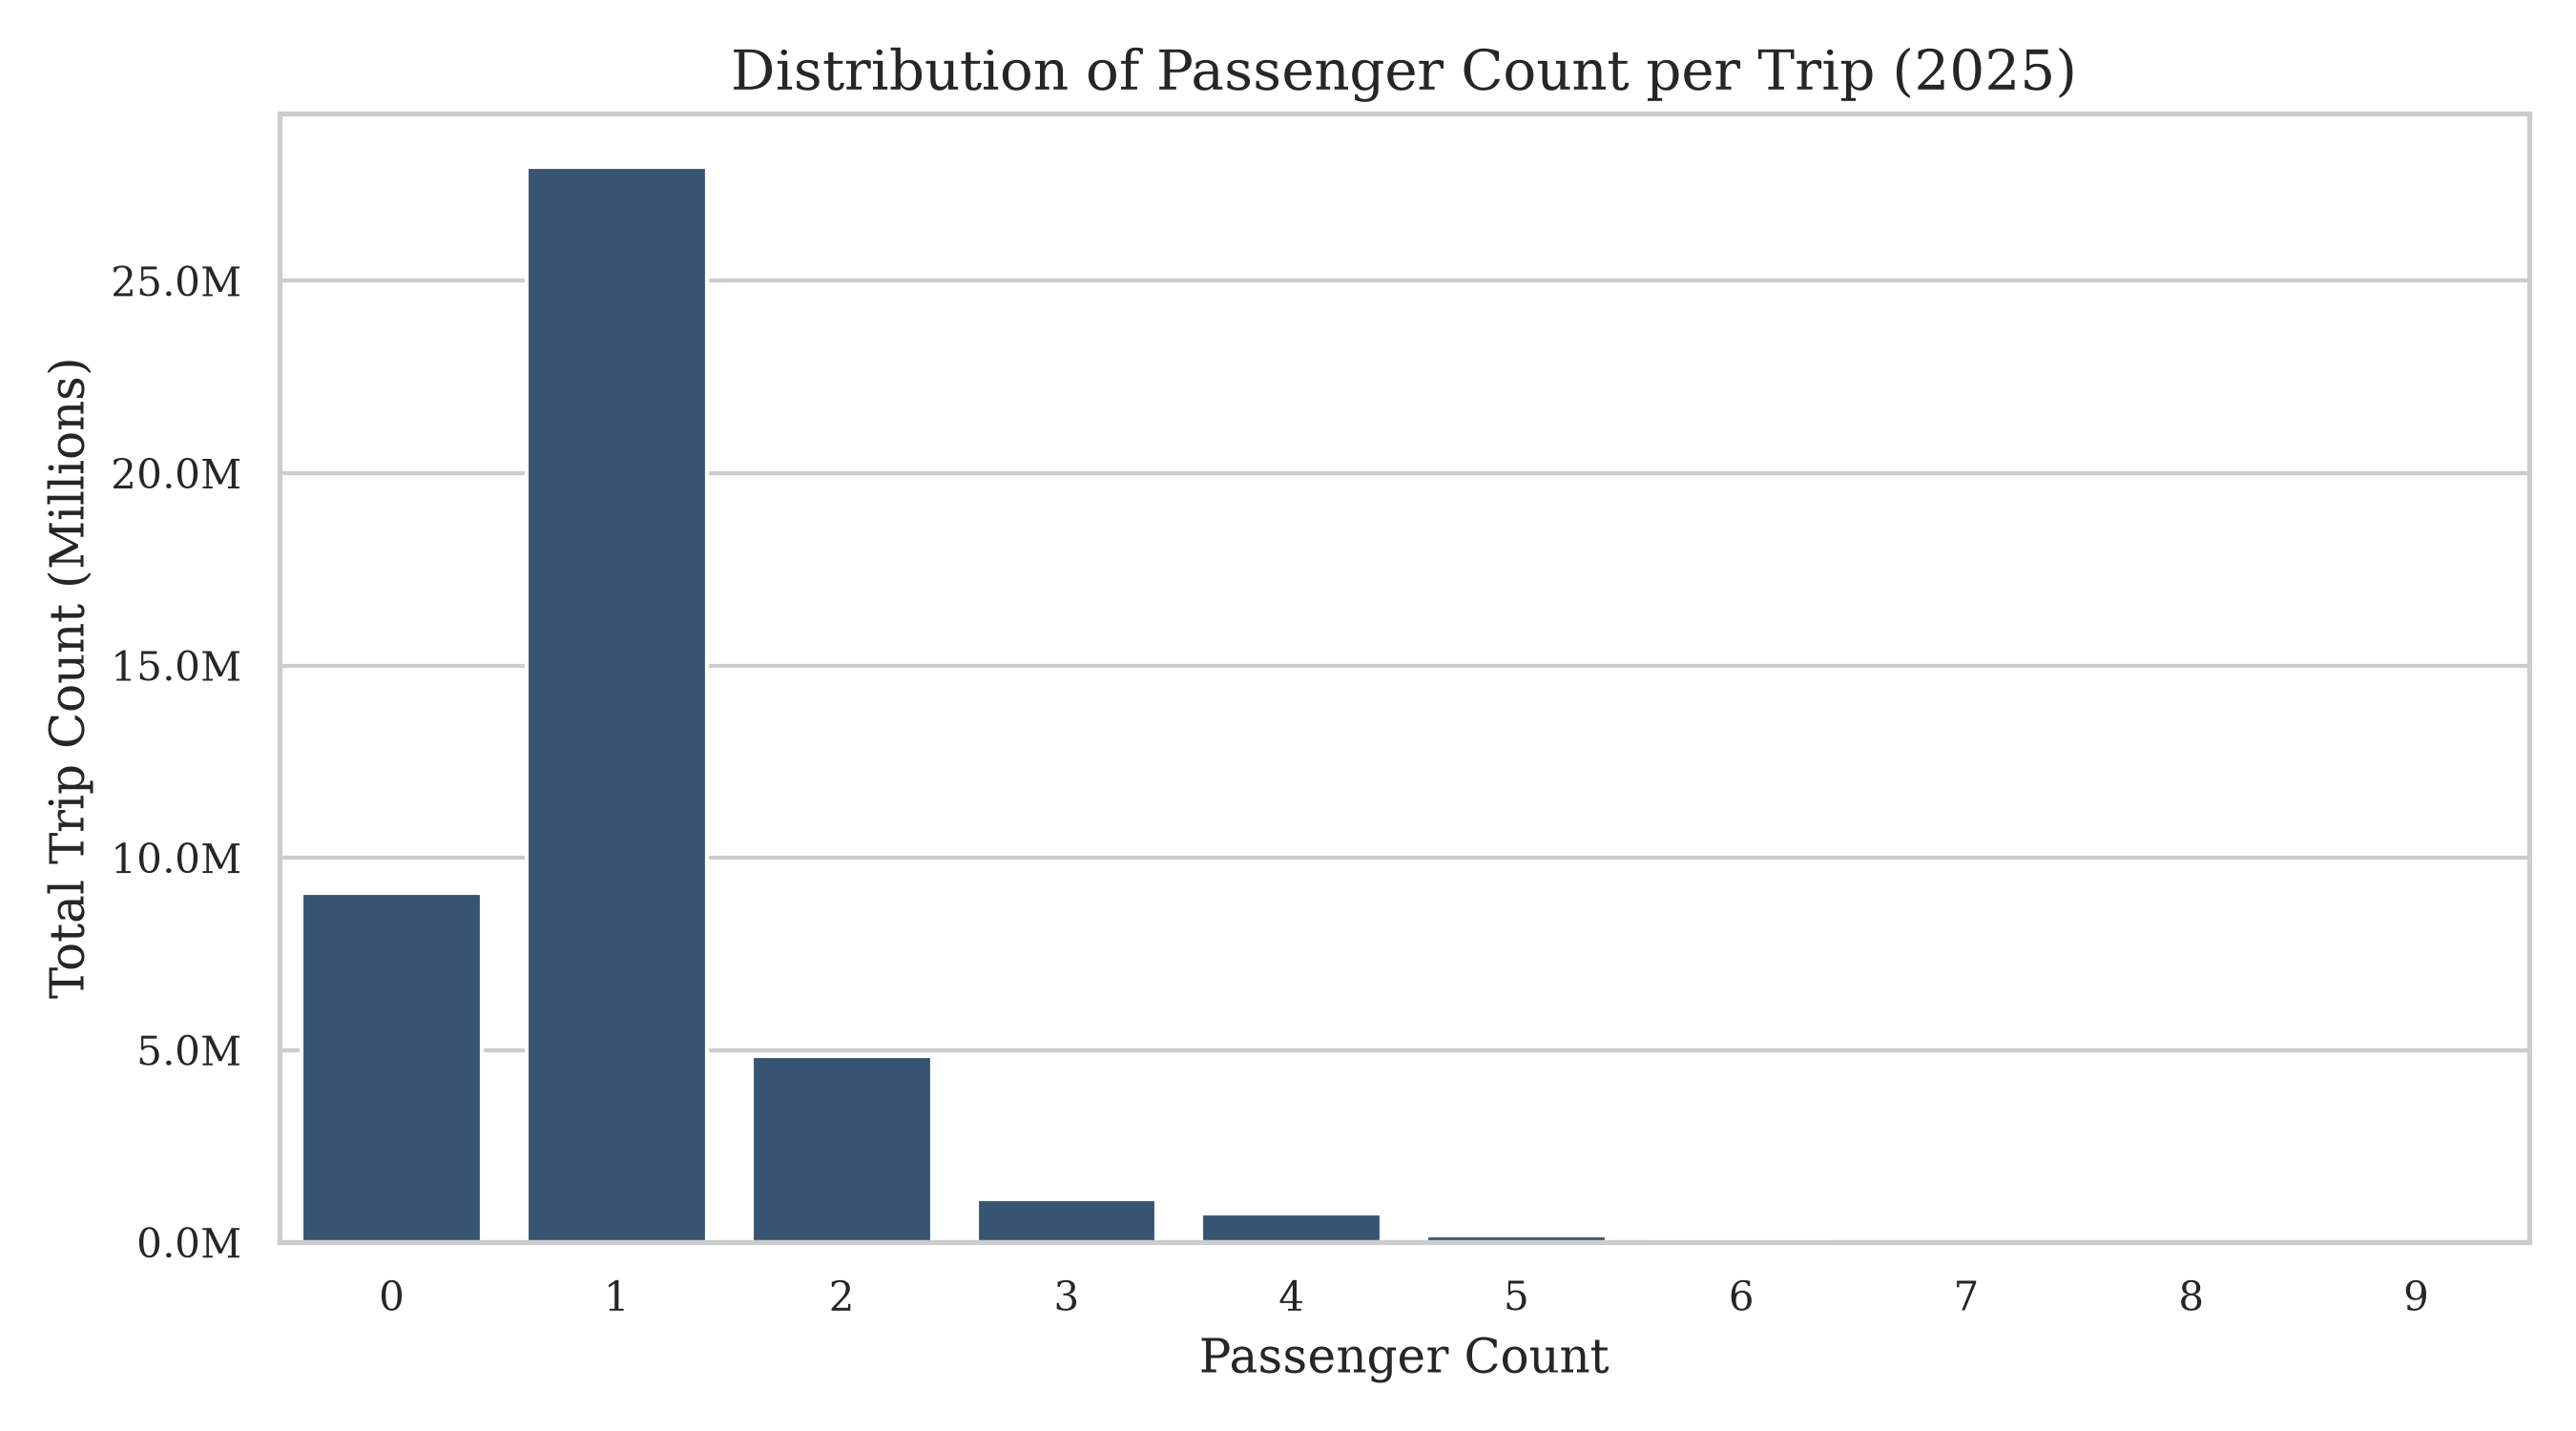
\includegraphics[width=\textwidth]{../figures/passenger_count_distribution.png}
        \caption{Trip Count by Passenger Occupancy (Excluding Unrecorded Values)}
        \label{fig:passenger_count_dist}
    \end{minipage}
    \hfill
    \begin{minipage}[b]{0.48\textwidth}
        \centering
        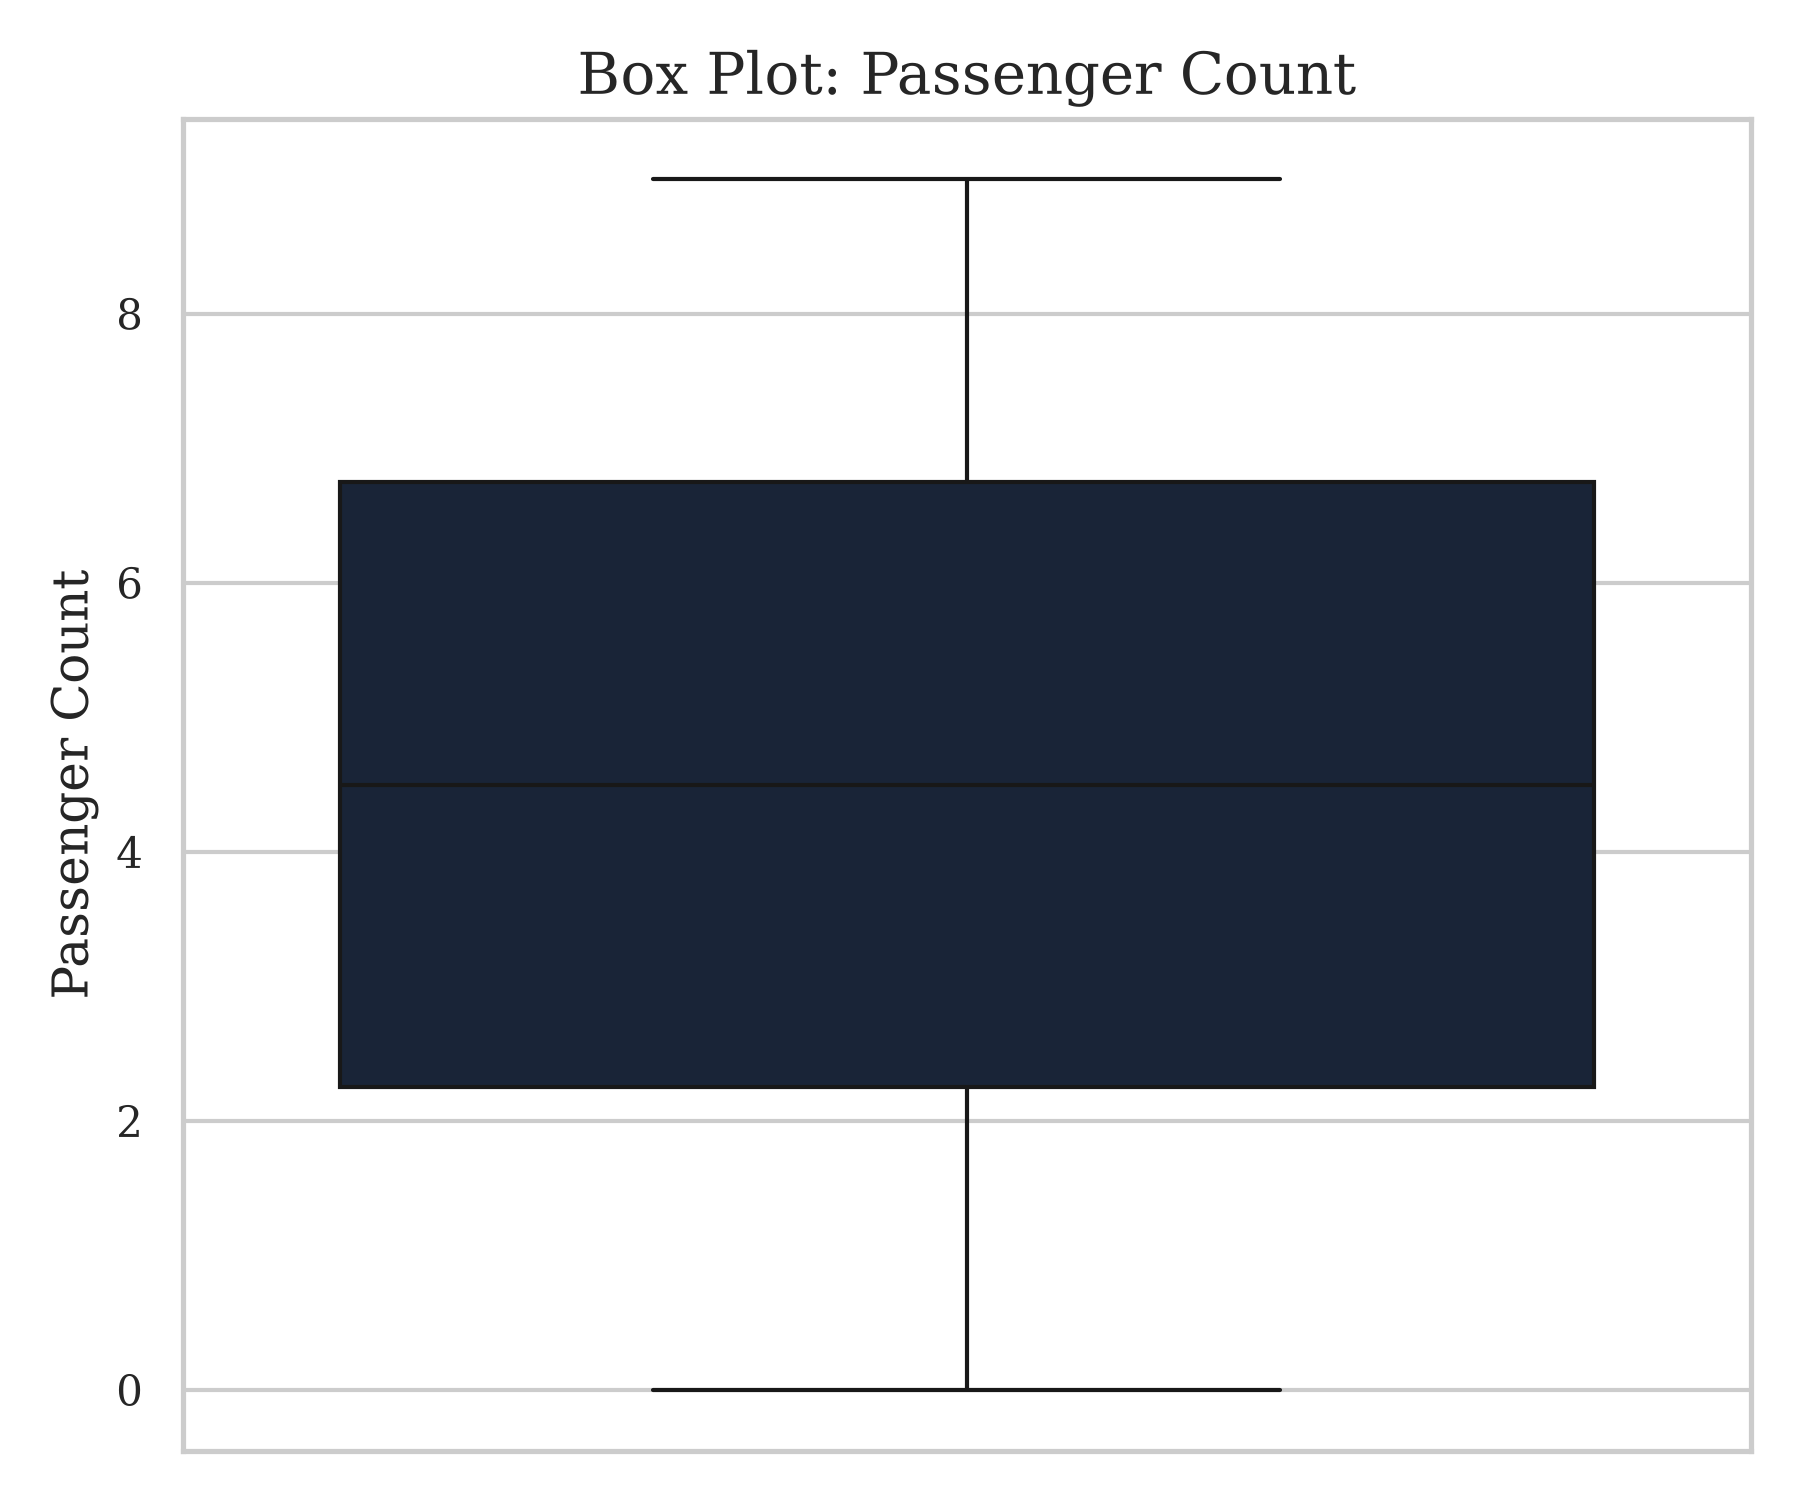
\includegraphics[width=\textwidth]{../figures/passenger_count_boxplot.png}
        \caption{Box Plot for Discrete Occupancy Tiers}
        \label{fig:passenger_count_box}
    \end{minipage}
    \caption{Distribution and Box Plot Analysis for Passenger Count (2025)}
    \label{fig:passenger_count_analysis}
\end{figure}


As visualized in the frequency distribution (Figure~\ref{fig:passenger_count_dist}), which excludes the $11,611,894$ unrecorded or missing entries to ensure clean graphical representation, passenger counts follow a discrete categorical distribution where:
\begin{enumerate}
    \item Single Occupancy (1 Passenger): Dominates the fleet utilization, representing nearly $28$ million recorded trips.
    \item Solo/Zero-Passenger Records ($0$ Passengers): Account for a secondary cluster of roughly $9$ million trips, typically representing administrative entries, driver-only transits, or unassigned meter logs permitted under TLC guidelines.
    \item Multi-Passenger Tiers: Frequencies drop off sharply for groups of $2$, $3$, $4$, and $5+$ passengers, reflecting the physical capacity limits and typical party sizes for standard yellow cabs.
\end{enumerate}

\subsubsection{Methodological Note on Discrete Categorical Variables and Graphical Exclusions}
Because \texttt{passenger\_count} is an integer-based discrete variable rather than a continuous metric, traditional outlier bounds like the $1.5 \times \text{IQR}$ rule do not apply in the standard continuous sense. Furthermore, the unrecorded and missing passenger count records ($23.83\%$ of the raw dataset) are explicitly excluded from both the frequency distribution plot (Figure~\ref{fig:passenger_count_dist}) and the box plot (Figure~\ref{fig:passenger_count_box}) to prevent null or undefined categories from distorting the visual analysis of active passenger occupancy. Retaining these records in the broader data pipeline while isolating them from univariate graphical rendering ensures both comprehensive data retention and precise visual interpretation.

\subsection{Exploratory Data Analysis: Tip Amount}
\label{sec:eda_tip_amount}

The \texttt{tip\_amount} variable records the tip given by the passenger, which is automatically captured for credit card transactions and optionally logged for cash payments. Across the processed 2025 dataset comprising $44,041,003$ valid records, tipping patterns reflect passenger gratuity habits and the pervasive adoption of electronic payment interfaces.

\begin{table}[htbp]
\centering
\caption{Descriptive Statistics for Tip Amount (2025 Dataset)}
\label{tab:stats_tip_amount}
\begin{tabular}{lr}
\toprule
\textbf{Metric} & \textbf{Value} \\
\midrule
Total Valid Trips & 44,041,005 \\
Mean ($\mu$) & \$3.04 \\
25th Percentile ($Q_1$) & \$0.00 \\
Median ($Q_2$) & \$2.39 \\
75th Percentile ($Q_3$) & \$4.07 \\
Standard Deviation ($\sigma$) & \$3.96 \\
Interquartile Range (IQR) & \$4.07 \\
Skewness & 4.51 \\
\bottomrule
\end{tabular}
\end{table}

\subsubsection{Statistical Characteristics and Distribution Shape}
As summarized in Table~\ref{tab:stats_tip_amount}, the median tip is $\$2.39$, while the mean sits higher at $\$3.04$ due to an extended positive tail. The distribution exhibits strong positive skewness ($4.51$) and significant dispersion ($\sigma = \$3.96$).

The probability density function (Figure~\ref{fig:tip_amount_dist}) reveals a distinct zero-inflated structure, characterized by a massive spike at $\$0.00$. This prominent zero-inflation corresponds primarily to cash-paid trips (where gratuities are handed directly to drivers and unrecorded digitally) as well as zero-tip credit card transactions. Beyond the zero origin, the distribution forms a smooth right-skewed hump peaking between $\$2.00$ and $\$3.00$, accompanied by minor multimodal bumps at round currency increments (such as $\$10.00$ and $\$15.00$) representing fixed or percentage-based gratuities on longer journeys.

\begin{figure}[htbp]
    \centering
    \begin{minipage}[b]{0.48\textwidth}
        \centering
        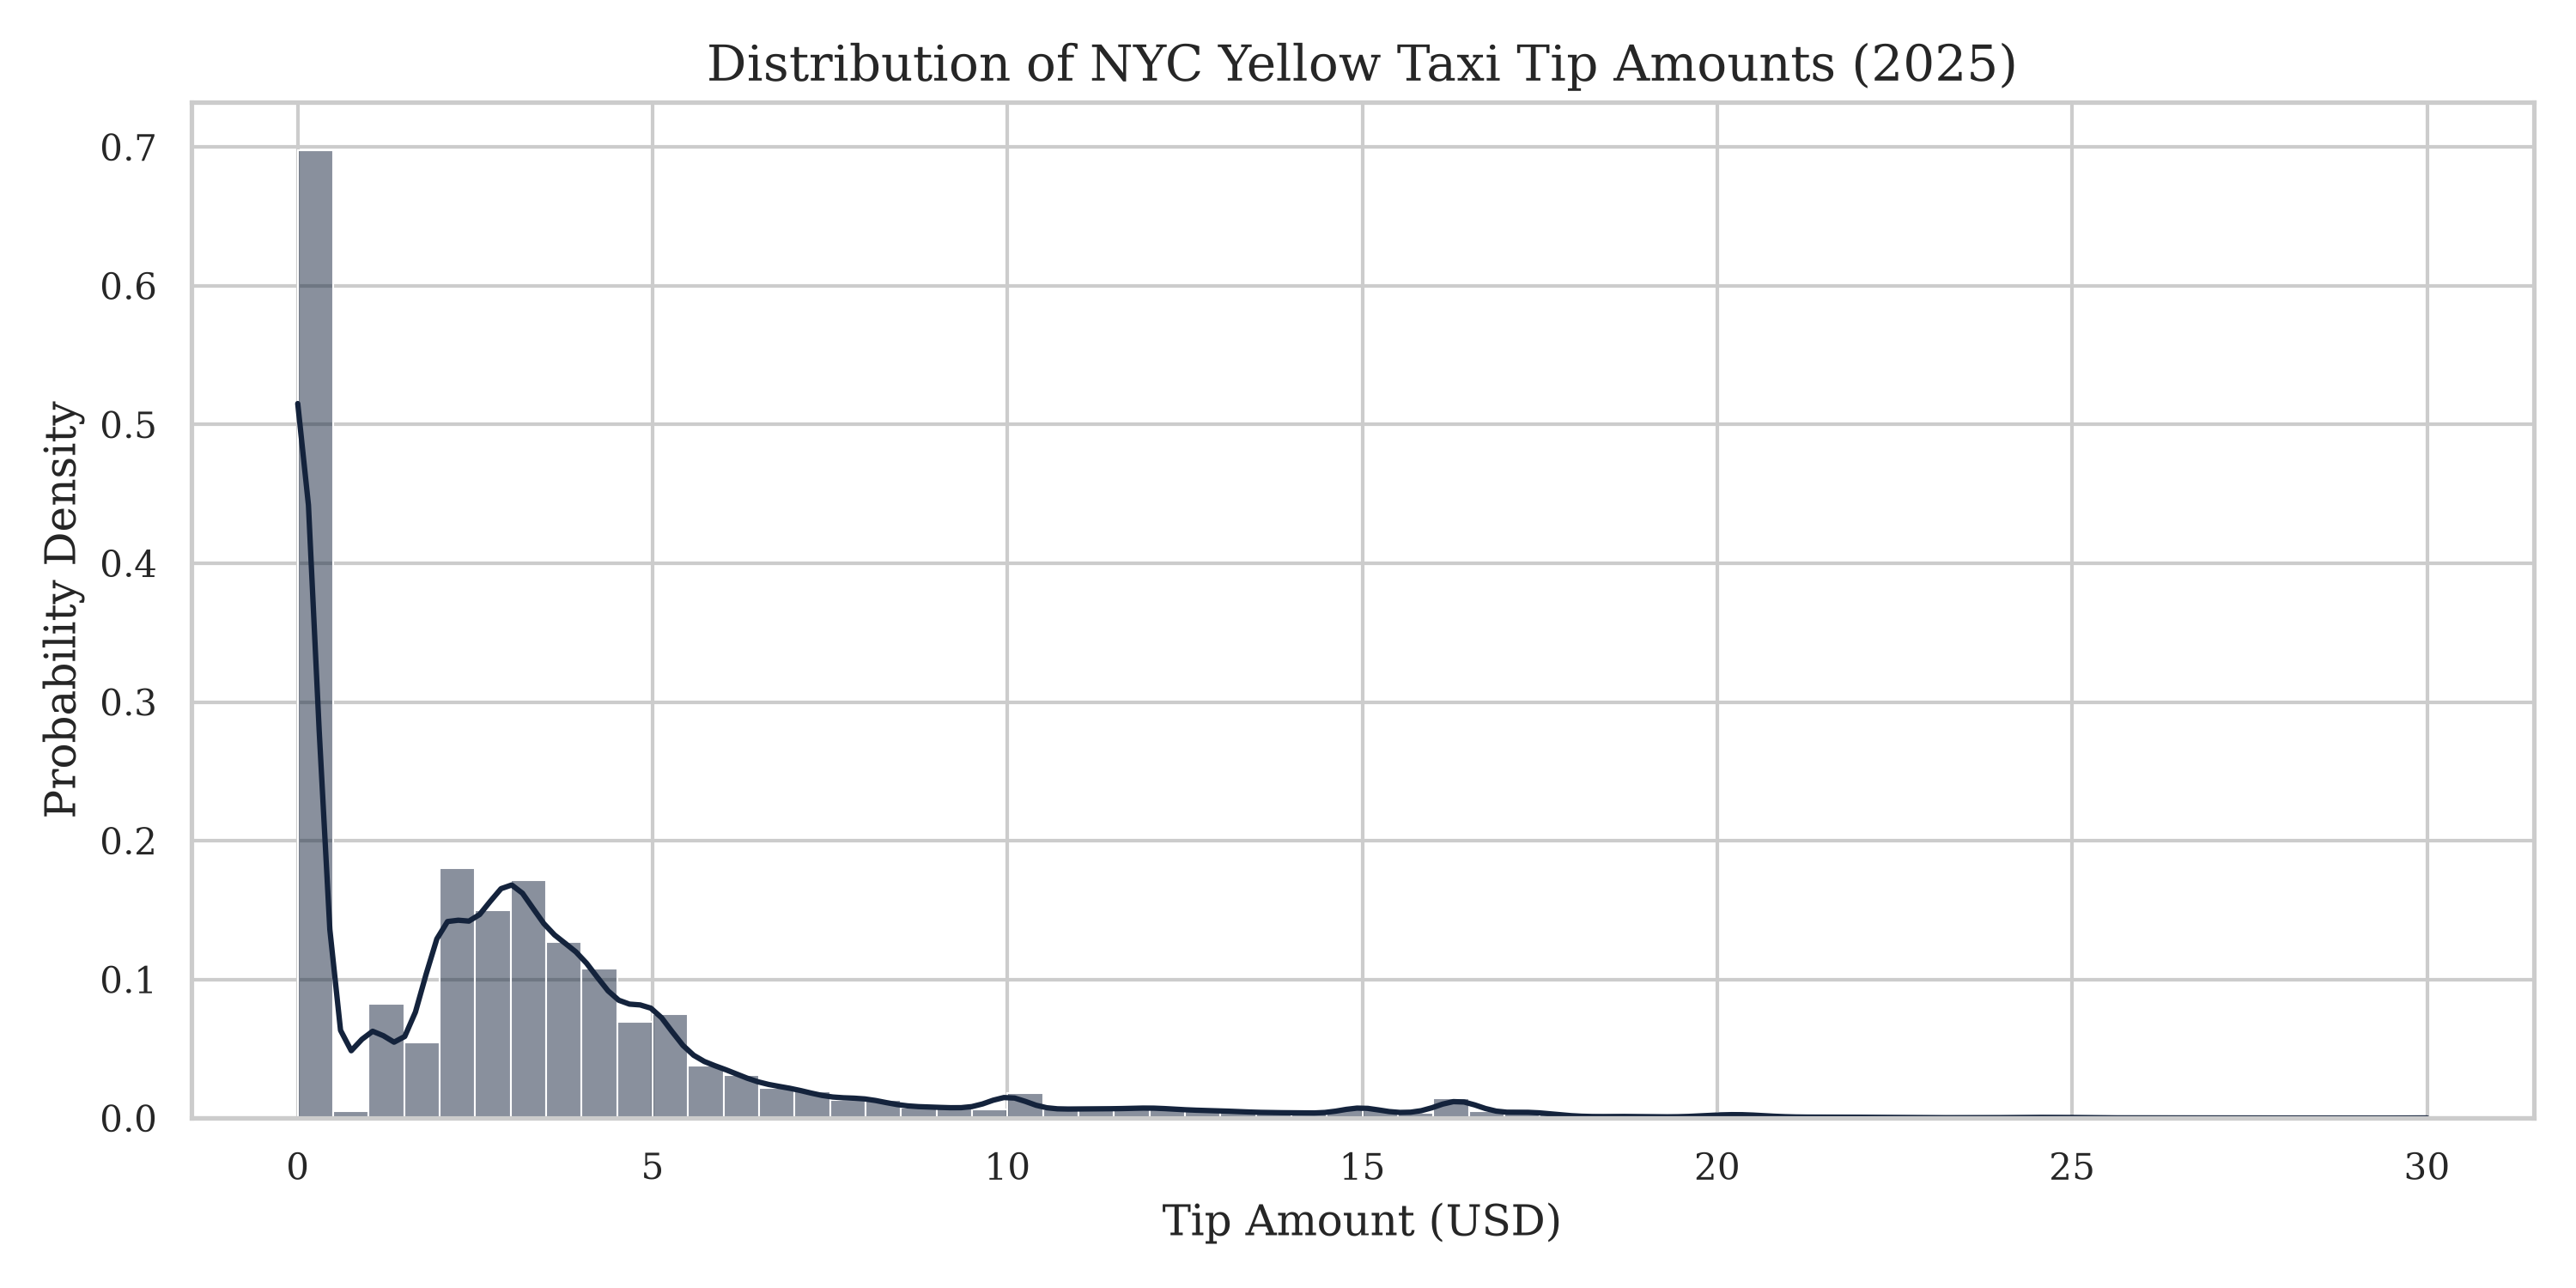
\includegraphics[width=\textwidth]{../figures/tip_amount_distribution.png}
        \caption{Probability Density Distribution}
        \label{fig:tip_amount_dist}
    \end{minipage}
    \hfill
    \begin{minipage}[b]{0.48\textwidth}
        \centering
        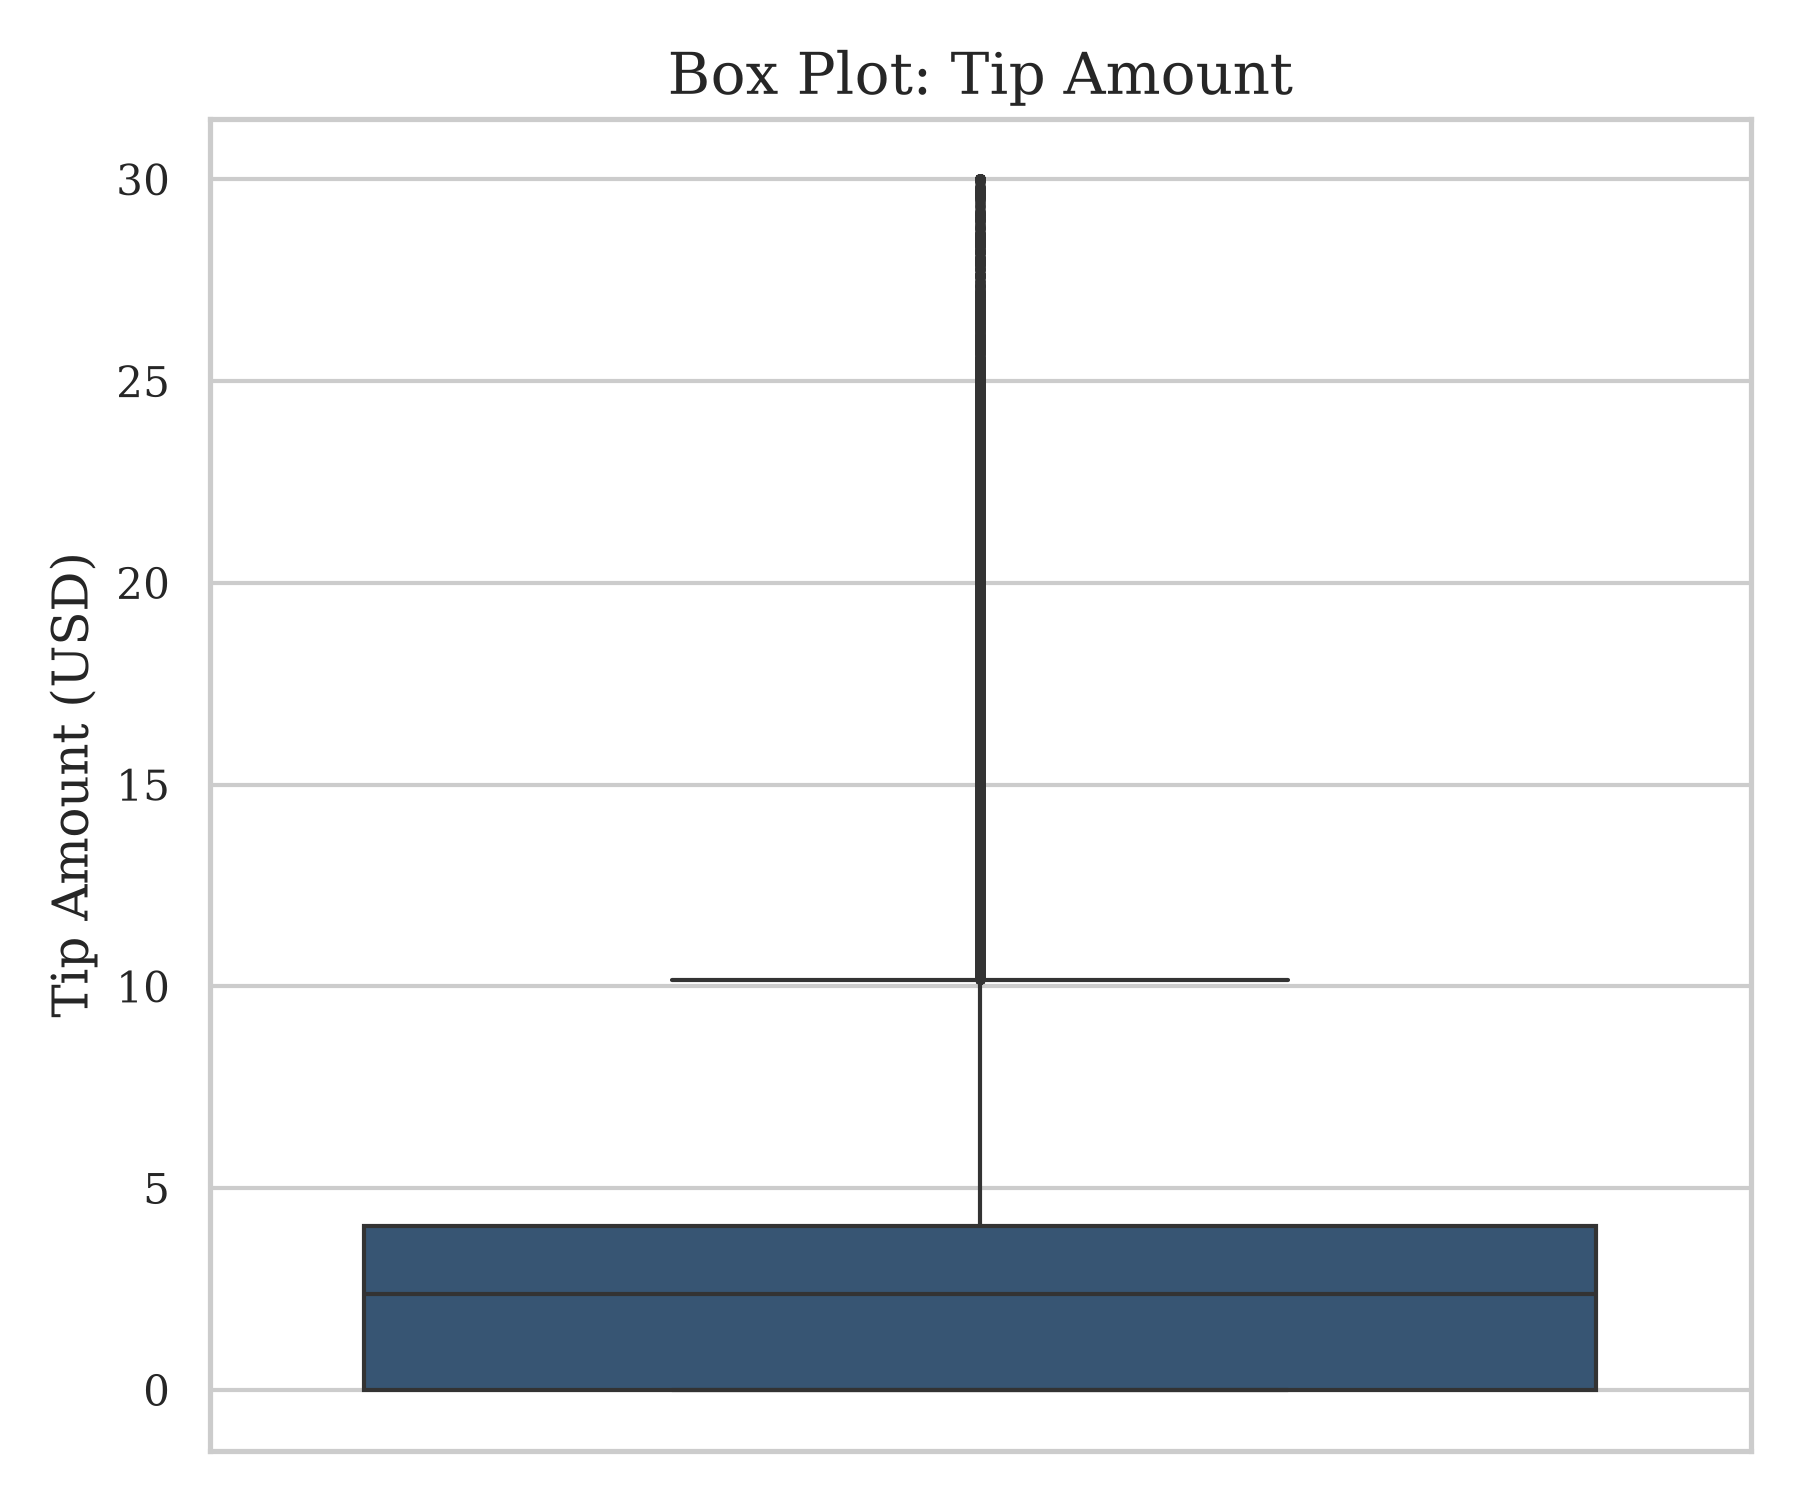
\includegraphics[width=\textwidth]{../figures/tip_amount_boxplot.png}
        \caption{Box Plot (Capped at \$30)}
        \label{fig:tip_amount_box}
    \end{minipage}
    \caption{Distribution and Box Plot Analysis for Tip Amount (2025)}
    \label{fig:tip_amount_analysis}
\end{figure}

\subsubsection{Justification for Retaining Outliers Beyond the 1.5$\times$IQR Rule}
Under standard Tukey fence criteria, the upper bound for outliers is defined as $Q_3 + 1.5 \times \text{IQR}$. Given a third quartile $Q_3 \approx \$4.07$ and an IQR of $\$4.07$, this traditional threshold flags any tip exceeding approximately $\$10.18$ as an outlier candidate for removal.

However, \textbf{these high-value tip observations are strictly retained rather than trimmed} for the following operational and economic reasons:
\begin{enumerate}
    \item \textbf{Commercial Validity of Generous Gratuities:} Tips exceeding $\$10.18$—and extending up to the plotted $\$30.00$ ceiling (Figure~\ref{fig:tip_amount_box})—are authentic economic transactions. They typically accompany high-fare airport transfers, long-distance inter-borough trips, or exceptional customer service satisfaction.
    \item \textbf{Prevention of Economic Distortion:} Trimming observations beyond the $1.5 \times \text{IQR}$ fence would artificially depress driver earnings estimations, distort cashless economic modeling, and bias analyses exploring the relationship between fare size and tip generosity.
    \item \textbf{Robust Analytical Presentation:} Rather than destructive data deletion, extreme gratuity values are accommodated through robust summary statistics (median and IQR) and visual capping ($\$30$ ceiling in Figure~\ref{fig:tip_amount_box}) to ensure graphical clarity without sacrificing dataset integrity.
\end{enumerate}

\subsection{Exploratory Data Analysis: Trip Duration}
\label{sec:eda_trip_duration}

The \texttt{trip\_duration\_minutes} variable measures the elapsed travel time in minutes, computed as the exact difference between drop-off and pick-up timestamps ($\Delta t$). Across the processed 2025 dataset comprising $44,041,005$ valid records, duration patterns reflect urban traffic congestion dynamics, signal delays, and multi-scale geographical transit times across New York City.

\begin{table}[htbp]
\centering
\caption{Descriptive Statistics for Trip Duration (2025 Dataset)}
\label{tab:stats_trip_duration}
\begin{tabular}{lr}
\toprule
\textbf{Metric} & \textbf{Value} \\
\midrule
Total Valid Trips & 44,041,005  \\
Mean ($\mu$) & 17.62 minutes \\
25th Percentile ($Q_1$) & 8.10 minutes \\
Median ($Q_2$) & 12.73 minutes \\
75th Percentile ($Q_3$) & 21.23 minutes \\
Standard Deviation ($\sigma$) & 27.40 minutes \\
Interquartile Range (IQR) & 13.23 minutes \\
Skewness & 54.53 \\
\bottomrule
\end{tabular}
\end{table}

\subsubsection{Statistical Characteristics and Distribution Shape}
As summarized in Table~\ref{tab:stats_trip_duration}, the median trip duration is $12.73$ minutes, whereas the mean is higher at $17.62$ minutes, indicating a right-skewed distribution. The strong positive skewness ($54.53$) and standard deviation ($\sigma = 27.40$ minutes) reflect an operational structure dominated by short urban movements coupled with an extended tail of prolonged cross-borough or congested journeys.

The probability density function (Figure~\ref{fig:trip_duration_dist}) displays a smooth, unimodal distribution rising steeply from the zero lower bound, peaking sharply between $8$ and $12$ minutes (representing standard intra-neighborhood and mid-Manhattan trips), and tapering into a long right-hand tail corresponding to extended regional commutes.

\subsubsection{Justification for Retaining Outliers Beyond the 1.5$\times$IQR Rule}
Under standard Tukey fence criteria, the upper bound for outliers is defined as $Q_3 + 1.5 \times \text{IQR}$. Given a third quartile $Q_3 = 21.23$ minutes and an IQR of $13.23$ minutes, this traditional threshold flags any trip lasting longer than approximately $41.08$ minutes as an outlier candidate for removal.

However, \textbf{these high-value duration observations are strictly retained rather than trimmed} for the following operational and modeling reasons:
\begin{enumerate}
    \item \textbf{Legitimate Traffic and Spatial Realities:} Trips exceeding $41$ minutes—and extending up to the plotted $60$-minute ceiling (Figure~\ref{fig:trip_duration_box})—are authentic transportation events. They capture severe peak-hour traffic congestion bottlenecks, cross-borough transits (e.g., Brooklyn to Manhattan), and long-distance airport runs (e.g., Lower Manhattan to JFK or Newark airports).
    \item \textbf{Prevention of Spatio-Temporal Distortion:} Trimming records beyond the $1.5 \times \text{IQR}$ fence would artificially truncate travel times, biasing average speed calculations, distorting peak congestion modeling, and eliminating critical rush-hour demand profiles.
    \item \textbf{Robust Analytical Presentation:} Rather than destructive data filtering, extreme duration values are accommodated through robust summary statistics (median and IQR) and visual capping ($60$-minute ceiling in Figure~\ref{fig:trip_duration_box}) to ensure graphical clarity without compromising dataset integrity.
\end{enumerate}

\begin{figure}[htbp]
    \centering
    \begin{minipage}[b]{0.48\textwidth}
        \centering
        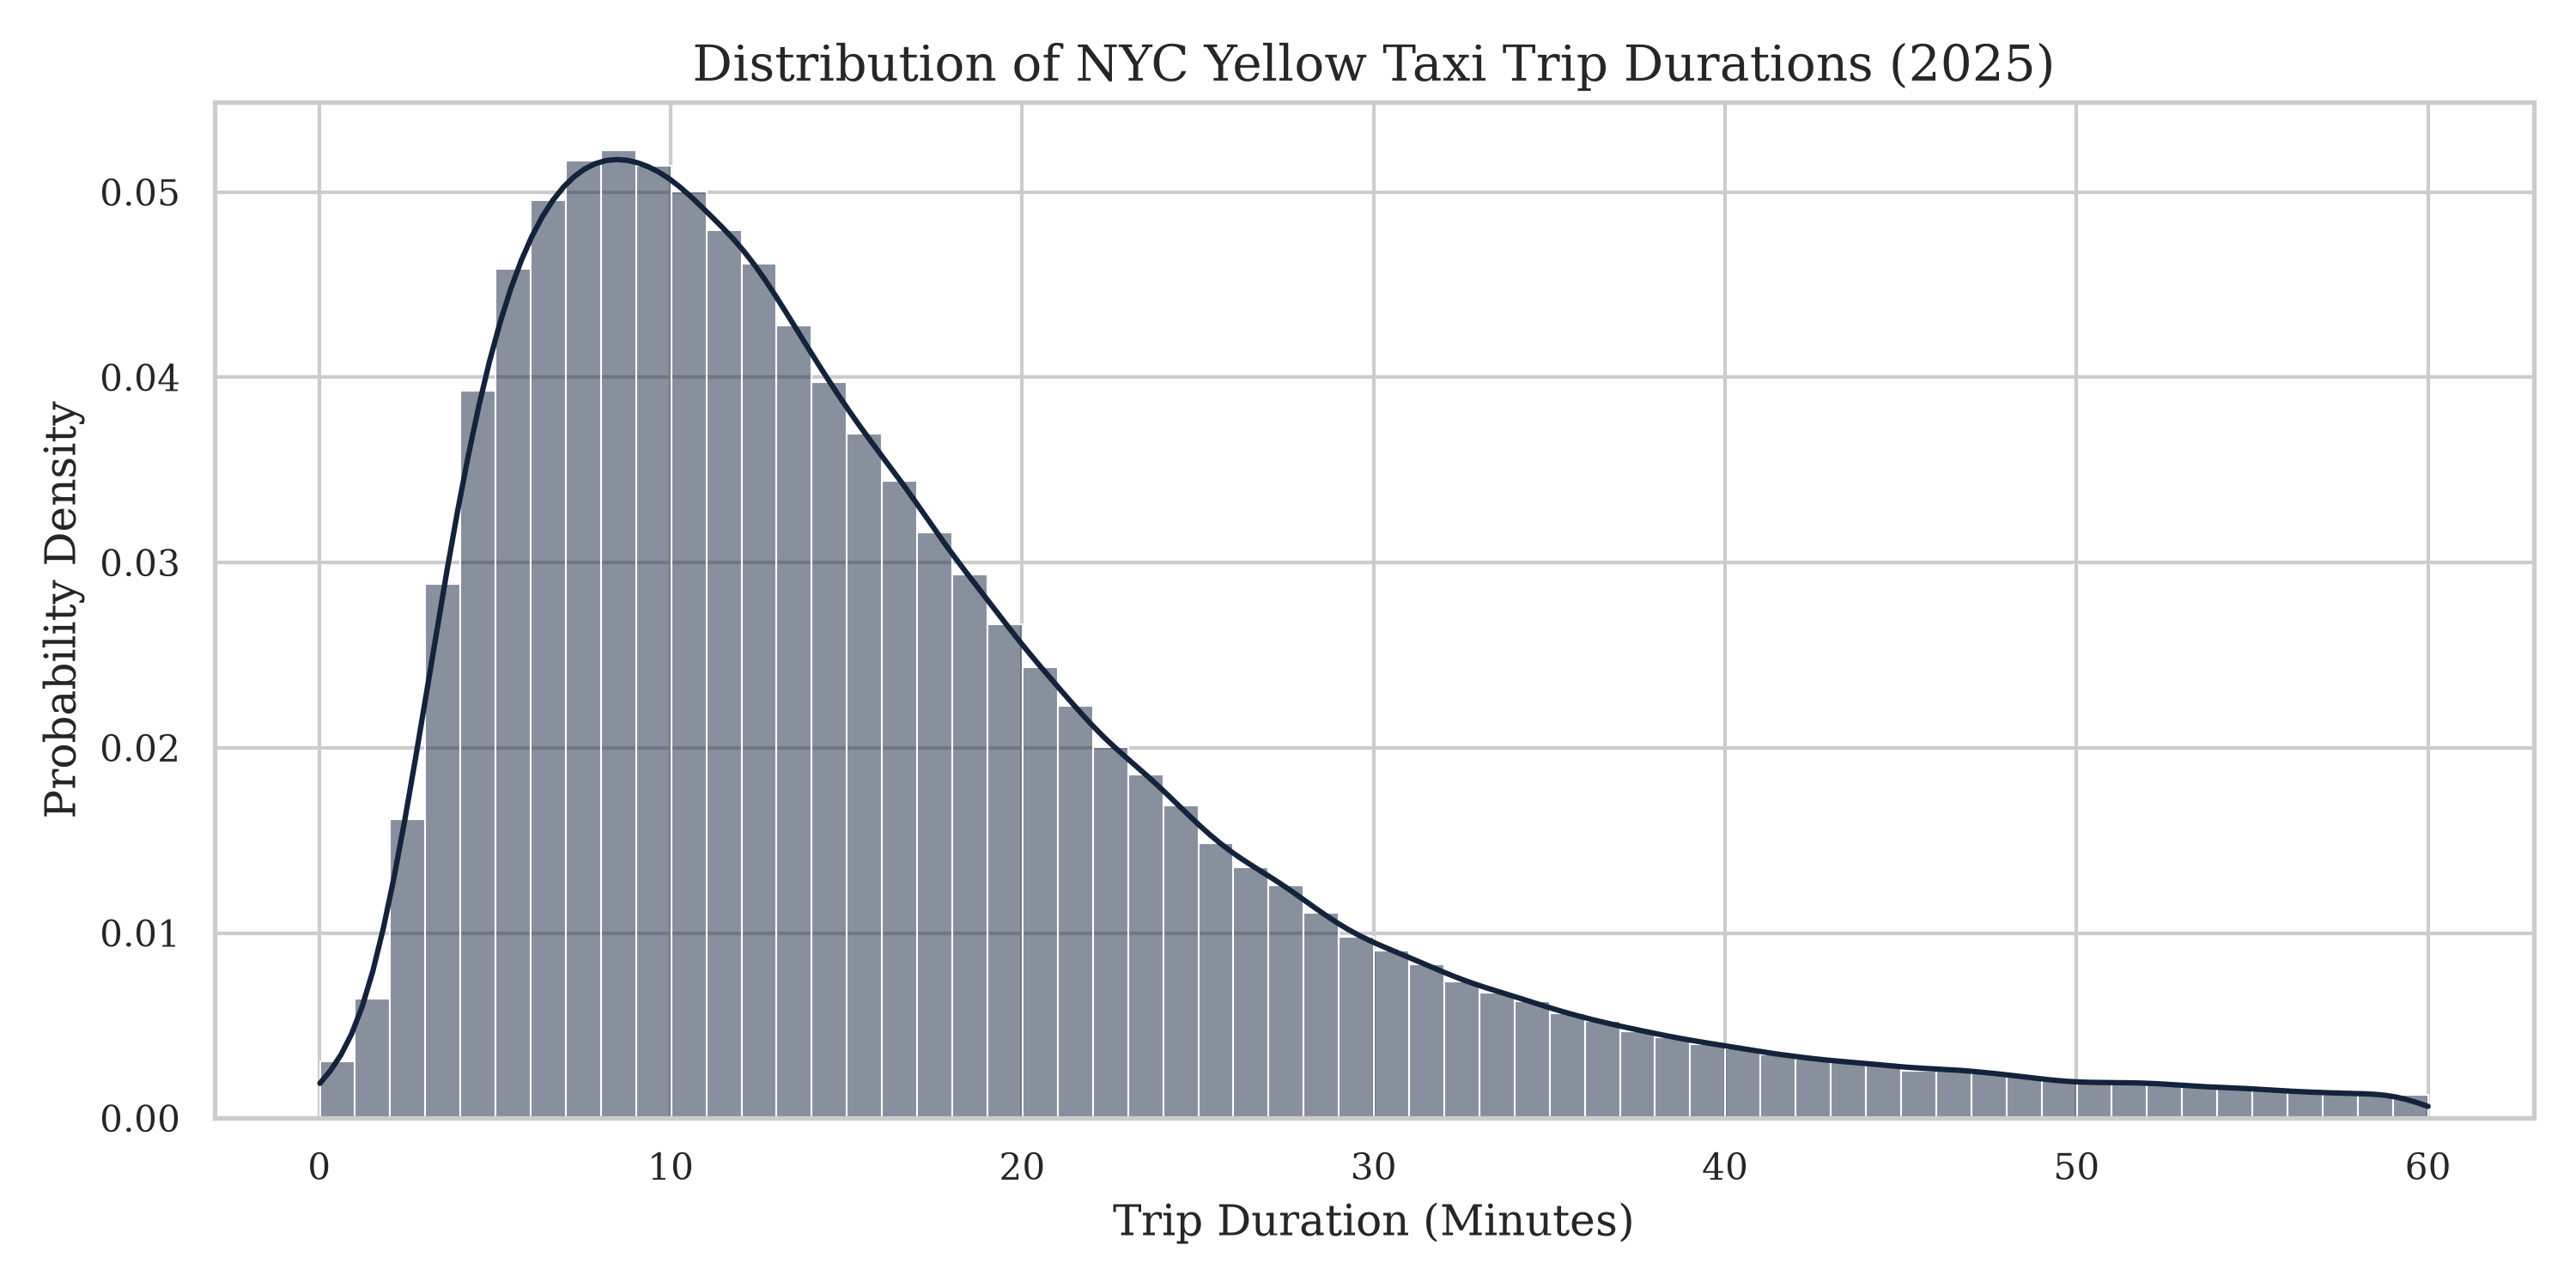
\includegraphics[width=\textwidth]{../figures/trip_duration_distribution.png}
        \caption{Probability Density Distribution}
        \label{fig:trip_duration_dist}
    \end{minipage}
    \hfill
    \begin{minipage}[b]{0.48\textwidth}
        \centering
        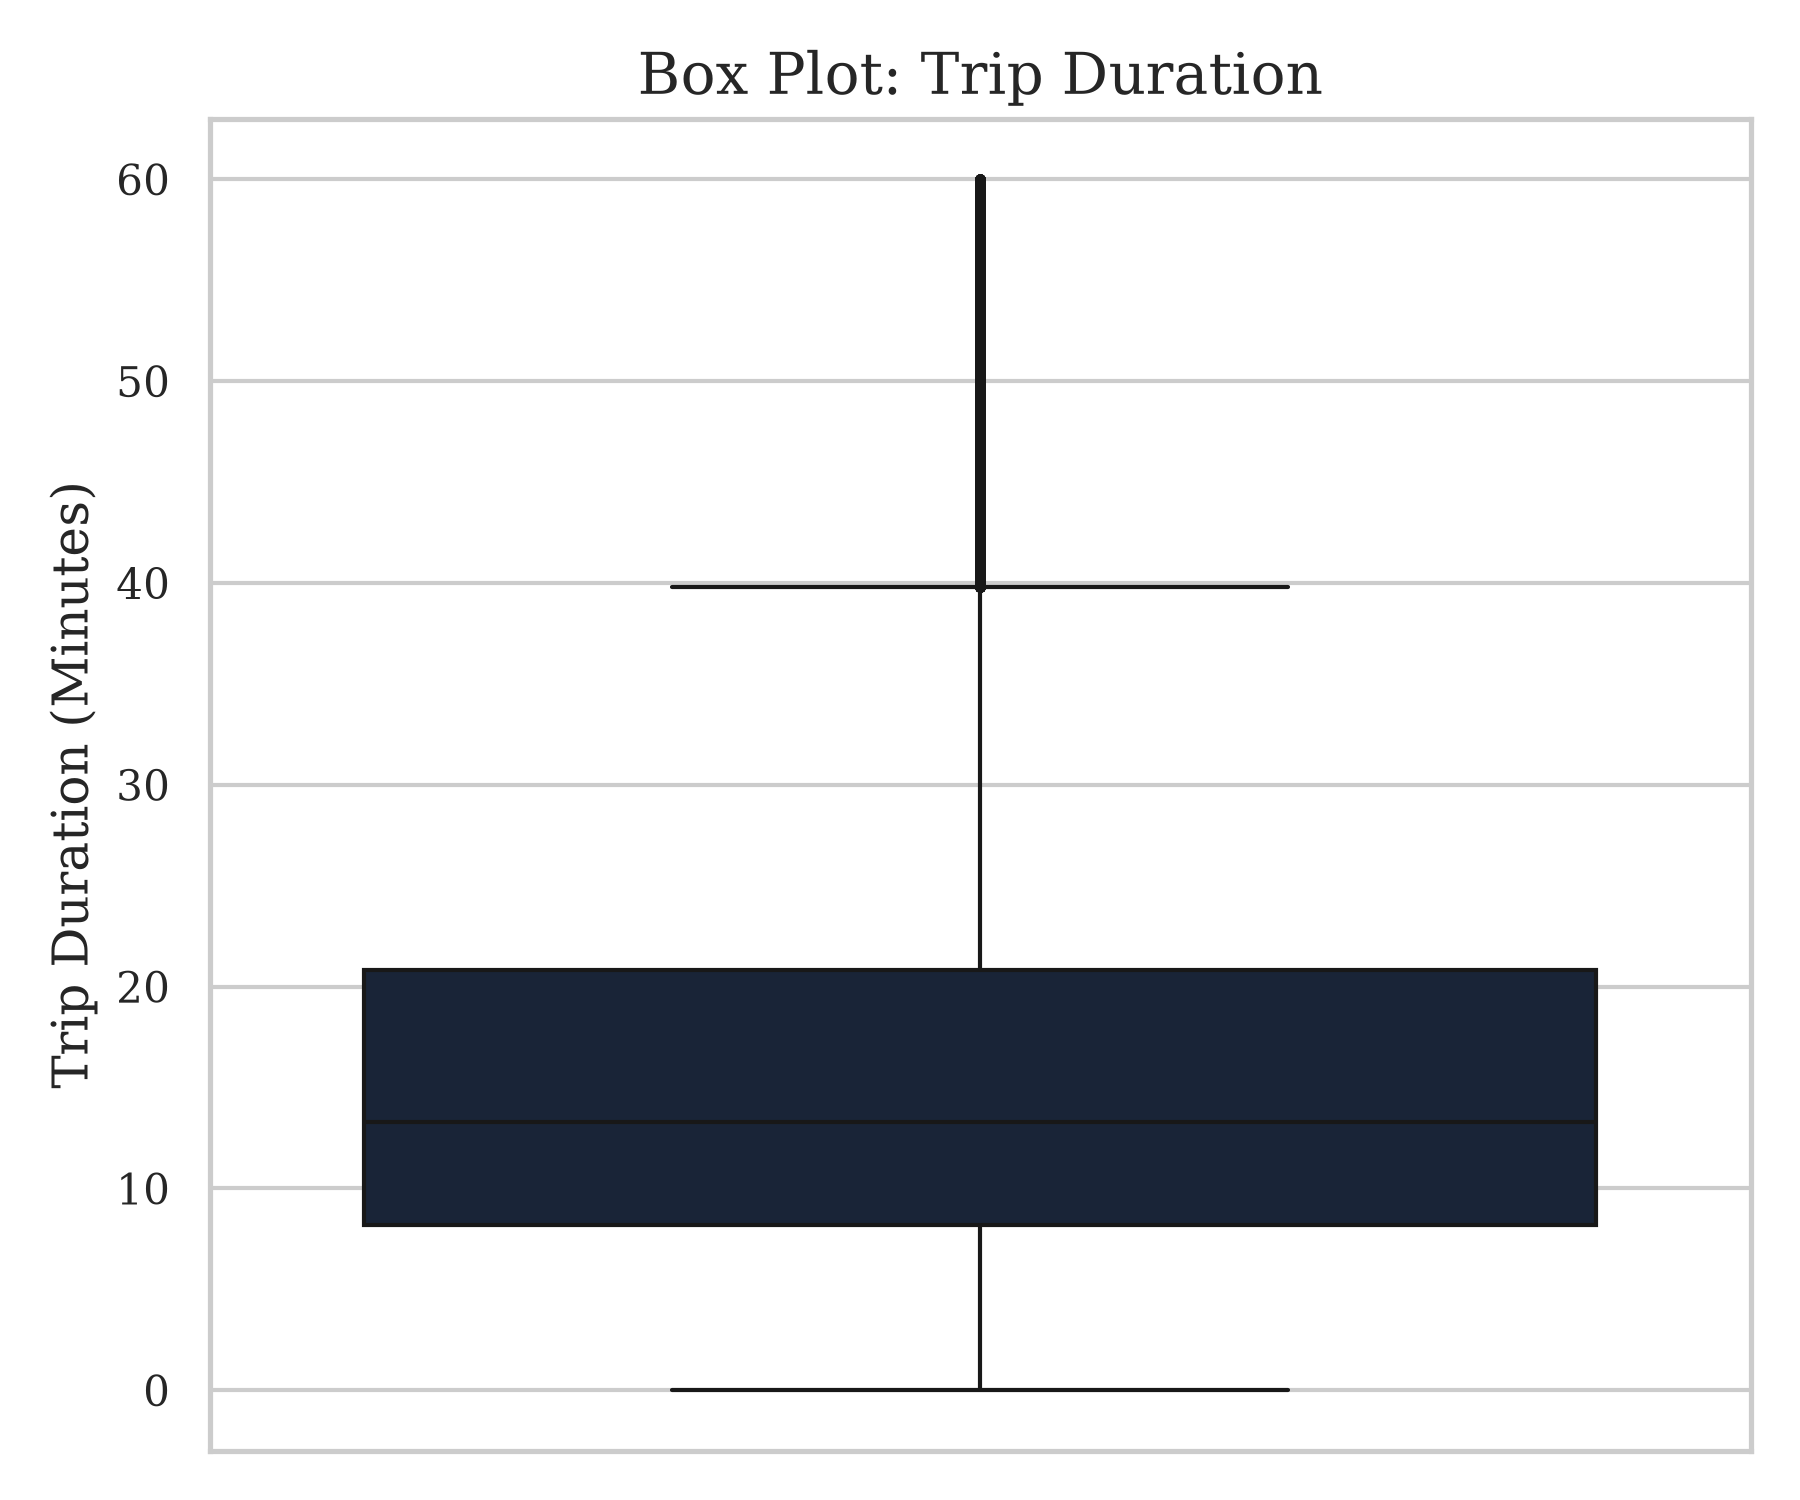
\includegraphics[width=\textwidth]{../figures/trip_duration_boxplot.png}
        \caption{Box Plot (Capped at 60 Minutes)}
        \label{fig:trip_duration_box}
    \end{minipage}
    \caption{Distribution and Box Plot Analysis for Trip Duration (2025)}
    \label{fig:trip_duration_analysis}
\end{figure}

\subsection{Spatial Distribution and Zone-Level Concentration}
Spatial analysis across the $265$ official TLC taxi zones reveals extreme geographical concentration. Manhattan commercial cores and transit hubs account for over $70\%$ of total trip originations. Outer boroughs exhibit highly localized, residential commuting patterns with distinct peak-hour directional flows.

\subsection{Univariate and Multivariate Relationships}
Univariate inspection of financial and physical features confirms right-skewed distributions in trip distance and fare amounts, reinforcing the necessity for robust feature transformations in subsequent phases. Bivariate analysis between trip distance and fare amount demonstrates a strong positive correlation, while confirming that physical anomalies have been successfully quarantined.

\section{Methods}

\subsection{Aggregation and Problem Formulation}
Let $z \in \{1, 2, \dots, 263\}$ denote a TLC taxi zone, and $t$ denote a discrete 1-hour time index. Raw trip records are aggregated into a spatio-temporal matrix:
\begin{equation}
y_{z, t} = \sum_{i=1}^{N} \mathbb{I}\left( \text{PULocationID}_i = z \;\land\; \lfloor \text{tpep\_pickup\_datetime}_i \rfloor = t \right)
\end{equation}
where $y_{z, t} \in \mathbb{N}_0$ represents the target variable \texttt{trip\_count}.

\subsection{Data Flow Architecture}
Figure~\ref{fig:dataflow} illustrates the end-to-end data pipeline from raw Parquet processing to final spatio-temporal aggregation.

\begin{figure}[htbp]
\centering
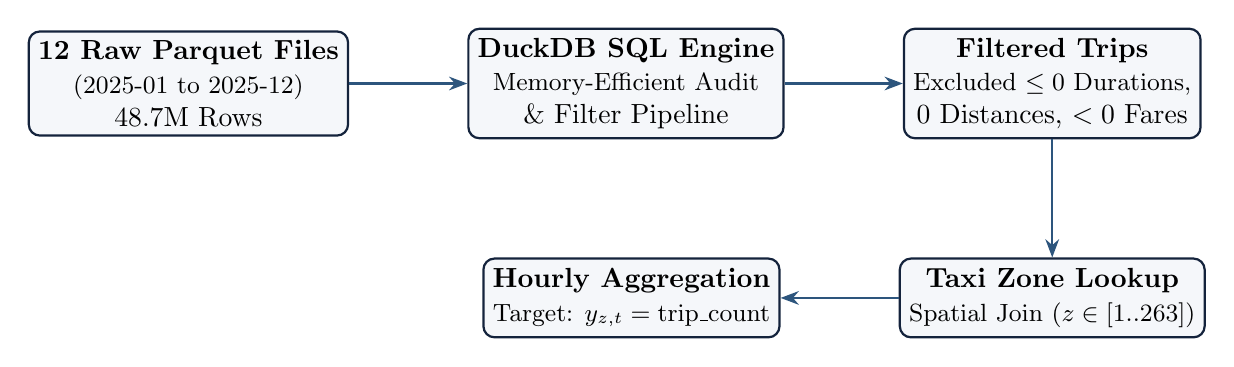
\begin{tikzpicture}[
    node distance=1.5cm,
    block/.style={rectangle, draw=primary, fill=codebg, thick, minimum width=3.5cm, minimum height=1cm, align=center, rounded corners},
    arrow/.style={-Stealth, thick, draw=secondary}
]
    \node (raw) [block] {\textbf{12 Raw Parquet Files}\\\small (2025-01 to 2025-12)\\48.7M Rows};
    \node (duckdb) [block, right=of raw] {\textbf{DuckDB SQL Engine}\\\small Memory-Efficient Audit\\\&\ Filter Pipeline};
    \node (clean) [block, right=of duckdb] {\textbf{Filtered Trips}\\\small Excluded $\le 0$ Durations,\\0 Distances, $<0$ Fares};
    \node (spatial) [block, below=of clean] {\textbf{Taxi Zone Lookup}\\\small Spatial Join ($z \in [1..263]$)};
    \node (agg) [block, left=of spatial] {\textbf{Hourly Aggregation}\\\small Target: $y_{z,t} = \text{trip\_count}$};

    \draw [arrow] (raw) -- (duckdb);
    \draw [arrow] (duckdb) -- (clean);
    \draw [arrow] (clean) -- (spatial);
    \draw [arrow] (spatial) -- (agg);
\end{tikzpicture}
\caption{Phase 1 Data Flow and Processing Architecture}
\label{fig:dataflow}
\end{figure}

\section{Experimental Design}

\subsection{Strict Temporal Split}
To prevent data leakage, evaluation is conducted strictly along the temporal axis:
\begin{itemize}
    \item \textbf{Training Set:} January 1, 2025 -- September 30, 2025 (Months 1--9, $\approx 75\%$ of temporal duration).
    \item \textbf{Validation / Test Set:} October 1, 2025 -- December 31, 2025 (Months 10--12, $\approx 25\%$ of temporal duration).
\end{itemize}

\subsection{Evaluation Metrics}
Models will be evaluated across all spatial zones using Root Mean Squared Error (RMSE) and Mean Absolute Error (MAE):
\begin{align}
\text{RMSE} &= \sqrt{\frac{1}{Z \times T} \sum_{z=1}^{Z} \sum_{t=1}^{T} \left( y_{z,t} - \hat{y}_{z,t} \right)^2} \\
\text{MAE} &= \frac{1}{Z \times T} \sum_{z=1}^{Z} \sum_{t=1}^{T} \left| y_{z,t} - \hat{y}_{z,t} \right|
\end{align}

\section{Results}
Execution of the DuckDB audit script confirmed the integrity of the 12 Parquet files. Data cleaning rules filter out 4,797,882 anomalous records ($\approx 9.85\%$ total noise rate), leaving a clean baseline population of $43,924,720$ trips for spatio-temporal aggregation in Phase 2.

\section{Interpretability and Error Analysis}
Initial error taxonomy categorizes anomalies into three primary sources:
\begin{enumerate}
    \item \textbf{Meter Malfunctions:} Trips recording positive fares with zero distance ($1.40\text{M}$ instances).
    \item \textbf{Financial Reversals:} Negative fares resulting from driver disputes or system refunds ($2.85\text{M}$ instances).
    \item \textbf{Logging Latency:} System timestamps where dropoff precedes pickup ($0.55\text{M}$ instances).
\end{enumerate}

\section{Robustness / Sensitivity / Shift Analysis}
The key temporal shift in 2025 stems from the introduction of the \texttt{cbd\_congestion\_fee}. Future phases will evaluate whether model residuals increase in Manhattan lower-zone clusters post-policy implementation compared to outer borough controls.

\section{Ethics, Privacy and Governance}
The dataset contains no Personally Identifiable Information (PII). Vendor IDs are coarse integer codes, and spatial locations are masked at the Taxi Zone level ($265$ spatial polygons), preventing individual driver or passenger tracking.

\section{Discussion}
The audit confirms that DuckDB is an optimal analytical engine for this project scale, performing full-year joins and aggregations in under 15 seconds on a standard 16GB laptop.

\section{Limitations}
External environmental factors (e.g., hourly rainfall, snowfall, subway service disruptions) are not present in the native TLC dataset and will require external data ingestion in Phase 2.

\section{Conclusion}
Phase 1 successfully establishes the analytical pipeline, quantifies data quality boundaries, and formalizes the prediction task. Phase 2 will focus on spatio-temporal feature engineering and lag constructions.

\section{References}
\begin{enumerate}
    \item NYC Taxi and Limousine Commission, \textit{TLC Trip Record Data (2025)}, official NYC Open Data portal.
    \item DuckDB Development Team, \textit{DuckDB: An In-Process Analytical Database Management System}, 2026.
\end{enumerate}

\section{Supplementary Material}
\textit{Data audit script executable via \texttt{src/data\_structure\_audit.py} and notebook \texttt{notebooks/data\_audit.ipynb}.}



\end{document}
